%\documentclass[10pt]{article}

\documentclass[aip,jcp,amsmath,amssymb, reprint]{revtex4-1}
%\documentclass[aip,jcp,amsmath,amssymb, linenumbers, reprint]{revtex4-1}
%\documentclass[aip,jcp,amsmath,amssymb, preprint]{revtex4-1}

\usepackage{graphicx}
\usepackage{dcolumn}
\usepackage{amsfonts}
\usepackage{braket}
\usepackage{multirow}
\usepackage{threeparttable}
\usepackage{xspace}
\usepackage{verbatim}
\usepackage{mhchem}
\usepackage{soul}
\usepackage{ulem}
\usepackage{siunitx}
\usepackage{lineno}% Enable numbering of text and display math
%\linenumbers\relax % Commence numbering lines
\usepackage[colorlinks = true,
            linkcolor = blue,
            urlcolor  = black,
            citecolor = blue,
            anchorcolor = black]{hyperref}

\usepackage{amsmath}
\usepackage{mathtools}
\usepackage{xcolor}
\usepackage{xspace}
\usepackage{ifthen}

\newcommand*{\Eh}{$E_{\rm h}$\xspace}
\newcommand*{\Ecorr}{$E_{\rm{corr}}$\xspace}
\newcommand*{\RCMnorm}{$\norm{\pmb{\lambda}_{2}}^{2}_\mathrm{F}$\xspace}
\newcommand*{\dRCMnorm}{$\norm{\pmb{\delta\lambda}_{2}}^{2}_\mathrm{F}$\xspace}
\newcommand*{\nfci}{N_\mathcal{H}}
\newcommand*{\ncomp}{\mathcal{V}_X}

\newcommand*{\gm}{\gamma}
\newcommand{\cop}[1]{\hat{a}^{\dagger}_{#1}}
\newcommand{\aop}[1]{\hat{a}_{#1}}

\providecommand{\norm}[1]{\lVert#1\rVert}

\setlength\linenumbersep{6pt}

\newcommand*\patchAmsMathEnvironmentForLineno[1]{%
  \expandafter\let\csname old#1\expandafter\endcsname\csname #1\endcsname
  \expandafter\let\csname oldend#1\expandafter\endcsname\csname end#1\endcsname
  \renewenvironment{#1}%
     {\linenomath\csname old#1\endcsname}%
     {\csname oldend#1\endcsname\endlinenomath}}% 
\newcommand*\patchBothAmsMathEnvironmentsForLineno[1]{%
  \patchAmsMathEnvironmentForLineno{#1}%
  \patchAmsMathEnvironmentForLineno{#1*}}%
\AtBeginDocument{%
\patchBothAmsMathEnvironmentsForLineno{equation}%
\patchBothAmsMathEnvironmentsForLineno{align}%
\patchBothAmsMathEnvironmentsForLineno{flalign}%
\patchBothAmsMathEnvironmentsForLineno{alignat}%
\patchBothAmsMathEnvironmentsForLineno{gather}%
\patchBothAmsMathEnvironmentsForLineno{multline}%
}

% Make this look more like JCP
\usepackage{newtxtext,newtxmath}
\usepackage[scaled=1.0]{helvet}
\usepackage[compact]{titlesec}
\usepackage{xcolor}
\usepackage{notes2bib}
\bibnotesetup{ note-name = , use-sort-key = false}
% Format section header
\titleformat{\section}
  {\normalfont\sffamily\bfseries}
  {\thesection.}{0.5 em}{\MakeTextUppercase}
\titlespacing{\section}{0pt}{12pt}{12pt}

\titleformat{\subsection}[block]
  {\normalfont\sffamily\bfseries}
  {\thesubsection.}{0.5 em}{}
\titlespacing{\subsection}{0pt}{12pt}{8pt}

\titleformat{\subsubsection}[block]
  {\normalfont\itshape\sffamily\bfseries\raggedright}
  {\arabic{subsubsection}.}{0.5 em}{}
\titlespacing{\subsubsection}{0pt}{8pt}{8pt}

\usepackage{xcolor}
\usepackage{ifthen}

% Toggle
\newboolean{shownotes}
\setboolean{shownotes}{true} % Change to false to hide notes

% Define a command for color-coded notes
\newcommand{\note}[2]{%
  \ifthenelse{\boolean{shownotes}}%
    {\textcolor{#1}{#2}}%
    {}%
}

\begin{document}

\title{Exploting Sparsity in Quantum Imaginary Time Evolution}
\author{Lita, Victor}
\affiliation{Department of General Engineering, California Polytechnic State University, San Luis Obispo, CA, 93410}
\author{Stair, Nicholas H.}
\email{nstair@calpoly.edu}
\affiliation{Department of Physics, California Polytechnic State University, San Luis Obispo, CA, 93410}

\begin{abstract}
This work explores methods for exploiting sparsity in the quantum imaginary time evolution (QITE) algorithm. Though many popular classical methods for treating highly-correlated electronic systems have emerged, the prohibitive scaling of the many-particle wavefunction often limits their applicability to large systems. Furthermore, adaptive hybrid quantum/classical methods are often limited by the cost of repeatedly solving nonlinear equations, resulting in intractable problems for $>$10 electron systems. As we enter the early-fault tolerant era of quantum computing, there is a growing need for methods which scale economically with system size. To address this need, we have introduced residual selection into the QITE algorithm, using an adaptive ansatz built from arbitrary-order particle-hole operators to reduce scaling costs. We demonstrate that this selected variant (sQITE) is more cost effective than fixed ansatz methods at ground and excited state energy estimation, and can even compete with methods employing gradient-based selection for certain molecular geometries. Additionally, we show that double-factorization of the residual vector and implementation of a DICE-like protocol drastically reduces circuit depths and accelerates convergence of the algorithm for challenging strongly-correlated systems.

\end{abstract}

\linenumbersep=24pt

\maketitle

\section{\label{sec:intro}Introduction}


In modern quantum chemistry, solving the Schrödinger equation efficiently for molecules with strongly correlated electrons remains an important open challenge.\cite{Laughlin2000TheTheory}
Here, “strong correlation” refers to scenarios where the energy required to promote electrons to higher orbitals rivals the Coulomb repulsion between them, resulting in electronic states that must be described by an extensive mixture of Slater determinants.\cite{Tew2007ElectronCorrelation, kutzelnigg2003theory}
This complexity is central to phenomena such as bond dissociation and photochemical reactions,\cite{Mok1996DynamicalAnd,Holmes2017ExcitedStates} as well as to the behavior of systems exhibiting molecular magnetism\cite{malrieu2014magnetic} and high-temperature superconductivity.\cite{Lee2007HighTemp}

Conventional single-reference methods, such as Configuration Interaction (CI) and Coupled Cluster (CC), which generally build excitations out of the Hartree–Fock (HF) determinant, often fail to capture these effects with sufficient accuracy.\cite{Sherrill1999TheConfiguration,bartlett2007coupled}
Additionally, if trying to capture excited state properties, popular classical approaches like time-dependent density functional theory (TD-DFT)\cite{runge1984density,casida1995time} and equation-of-motion coupled cluster (EOM-CC)\cite{stanton1993equation} often falter in the presence of near-degenerate states, such as those occurring at avoided crossings and conical intersections.\cite{dreuw2004failure,krylov2008equation}

Although methods that can accurately treat strong correlation do exist—namely, the complete active space (CAS) family,\cite{Roos:1980wj} density matrix renormalization group (DMRG),\cite{White1992DensityMatrix} selected configuration interaction (CI),\cite{Huron1973IterativePerturbation,Buenker1974IndividualizedConfiguration} and multireference coupled cluster (MRCC) methods\cite{vcivzek1969use,lindgren1978coupled,jeziorski1981coupled,lyakh2012multireference, kohn2013state, evangelista2018perspective}—these approaches are computationally expensive, especially as they approach the full configuration interaction (FCI) limit.
Notably, while single-reference methods scale more favorably, they are often inaccurate in strongly correlated regimes, and multireference methods, though more accurate, incur significantly higher memory and computational costs, rendering them impractical for all but the smallest active spaces or highly specialized applications.\cite{piecuch1990coupled, piecuch2005renormalized,Limacher2013NewMean,Bulik2015CanSingle}

%In modern electronic structure theory, a major challenge is solving the many-body Schr\"odinger equation for strongly correlated electrons.\cite{9,10} The availability of accurate methods for these systems is imperative for understanding a myriad of important phenomena such as bond breaking and photochemical processes,\cite{1,2} molecular magnetism,\cite{3} high-temperature superconductivity,\cite{4} and others.\cite{5,6,7,8} In brief, strong correlation arises when the cost of promoting electrons to higher energy orbitals is comparable to the electron pairing (Coulombic) repulsion, causing the wave function to acquire nontrivial contributions from many Slater determinants,\cite{9,10} which single-reference treatments cannot effectively capture with a polynomial number of parameters. Consequently, accurately determining both ground and excited states of such systems remains one of the foremost challenges in electronic structure theory.\cite{4,5,6,7,8,9,10,11,36-44,57-60,61,62} Molecules and materials containing transition metals or highly conjugated frameworks frequently exhibit near-degenerate scenarios such as avoided crossings or conical intersections,\cite{1,2,3,8,9,10} for which classical single-reference approaches, including time-dependent density functional theory (TD-DFT)\cite{4,5} and the equation-of-motion coupled cluster (EOM-CC)\cite{6,7} hierarchy, often struggle to achieve quantitative accuracy when higher-than-double excitations dominate. Although multireference methods like the complete active space (CAS) family can in principle capture the requisite static correlation, their computational cost grows combinatorially with the number of electrons and orbitals, leading to prohibitively large parameter spaces for full configuration interaction (FCI). Consequently, classical approaches typically resort to approximate or selected-configuration procedures to reduce this burden, albeit with trade-offs in accuracy or the need for specialized truncation strategies.\cite{11,12-18,19-28,29-35,36-44,46-56,57-60,61,62}
%\textcolor{red}{Re-word too close to phrasing in exploring hilbert space}


%An outstanding challenge in modern electronic structure theory is solving the many-body Schr\"odinger equation for systems with strongly 
%correlated electrons.\cite{9,10} The availability of accurate computational methods for these systems is imperative for understanding 
%a myriad of important phenomena, including bond breaking and photochemical processes,\cite{1,2} molecular magnetism,\cite{3} 
%high-temperature superconductivity,\cite{4} and others.\cite{5,6,7,8} In brief, strong correlation arises when the cost of promoting 
%electrons to higher energy orbitals is comparable to the electron pairing (Coulombic) repulsion, rendering a mean-field picture 
%inadequate. Consequently, the wave function may acquire nontrivial contributions from many Slater determinants,\cite{9,10} 
%and single-reference treatments cannot effectively approximate such states with a polynomial number of parameters.
%
%Finding accurate ground and excited states of these strongly correlated systems thus remains one of the foremost challenges 
%in electronic structure theory.\cite{4,5,6,7,8,9,10,11,36-44,57-60,61,62} Molecules and materials containing transition metals or 
%highly conjugated frameworks frequently exhibit multireference character in their low-lying excited states and often present 
%near-degenerate scenarios such as avoided crossings or conical intersections.\cite{1,2,3,8,9,10} Classical single-reference 
%approaches, including time-dependent density functional theory (TD-DFT)\cite{4,5} or the equation-of-motion coupled cluster 
%(EOM-CC)\cite{6,7} family, typically struggle in these regimes, especially when higher-than-double excitations dominate. 
%Multireference methods like the complete active space (CAS) family can in principle capture the requisite static correlation, 
%but their computational cost grows combinatorially with the number of electrons and orbitals, leading to prohibitively large 
%parameter spaces for full configuration interaction (FCI). Consequently, classical approaches frequently resort to approximate 
%or selected-configuration procedures to reduce this burden, albeit with trade-offs in accuracy or the need for specialized 
%truncation strategies.\cite{11,12-18,19-28,29-35,36-44,46-56,57-60,61,62}



Quantum computational algorithms offer a compelling solution to at least the storage issue associated with the exponential number of FCI determinants by placing the many-particle wave function into a register of qubits.\cite{Abrams:1997ha,kassal2011simulating} 
Harnessing quantum-mechanical resources in this way holds the potential for more efficient description of strongly correlated electronic states in particular, as they are generally less amenable to classical compression or approximate representation. 
Significant progress in developing quantum-classical hybrid methods for ground- and excited-state electronic structure has emerged in recent years, either as stand alone algorithms or as state-preparation methods for quantum phase estimation (QPE).\cite{Abrams:1999ur}
Variational (VQE)\cite{Peruzzo:2014kca, yung2014transistor, McClean:2016bs, grimsley2019adaptive} and projective (PQE)\cite{stair2021simulating} quantum eigensolver approaches, which optimize the parameters of an ansatz circuit on classical hardware, have shown promise on today's noisy devices,\cite{OMalley:2016dc, colless2018computation, shen2017quantum, hempel2018quantum, nam2020ground} but face complications associated with high-dimensional, nonlinear optimizations that can easily become trapped in local minima. 
By contrast, imaginary time evolution (ITE) has a long history in classical simulations of correlated fermionic systems,\cite{feynman1948space,ceperley1980ground,sugiyama1986auxiliary,zhang1997constrained,foulkes2001quantum} and its quantum analogue (QITE) has been introduced\cite{motta2019determining} to obviate many of the classical optimization challenges. 
%Recent developments have demonstrated the efficacy of QITE,\cite{17-24} and combined with quantum Lanczos diagonalization (QLanczos)\cite{19,33} or the folded spectrum method, QITE has emerged as a promising algorithmic framework for extracting not only ground states but also excited states on near-term and early fault-tolerant quantum devices.
Recent advances in QITE have focused on reducing resource demands and accelerating convergence for both ground and excited state preparation, via QITE's Lanczos~\cite{motta2019determining} and/or Folded Spectrum (FS) formulations.\cite{Tsuchimochi2023Improved,McClean:2016bs,santagati2018witnessing,zhang2021adaptive}
A stochastic variational QITE approach significantly reduces measurement overhead on large-scale devices,\cite{gacon2023stochastic} while step-merging techniques have been successfully applied to combinatorial optimization problems such as MaxCut.\cite{gomes2020efficient,alam2023solving}
Composite formulations that extend qDRIFT-based methods into the imaginary-time regime offer rigorous error bounds and improved circuit efficiency.\cite{pocrnic2024composite, hagan2023composite} 
QITE has also been applied to diverse domains, including nuclear density functional theory\cite{li2024quantum} and molecular systems. Recently, Tsuchimochi~\textit{et. al.}~\cite{Tsuchimochi2023Improved} improved the derivation of the QITE equations in second quantization to enable larger time steps and reduced circuit depth.
In addition, alternative strategies based on drifting real-time evolution have lowered gate count and measurement complexity.\cite{huang2023efficient} 
Finally, adaptive variational QITE techniques and reinforcement learning-assisted QITE variants bridge QITE and variational approaches, further enhancing ground state preparation on near-term quantum devices.\cite{gomes2021adaptive,cao2022quantum}

With only the notable exception of Gomes~\textit{et. al.},~\cite{gomes2021adaptive} virtually all current QITE implementations rely on a \textit{fixed} pool of anti-Hermitian operators $\mathcal{A}$ to approximate the imaginary time propagation at each time step.
\note{blue}{Even in this case however, the selection still does not have access to the global oprator pool and is inherently limited. better than pqe cause no nonlinear solve and natural connection between residual magnitudes in full pool and operator magnitudes.}
The dimension of $\mathcal{A}$ directly dictates both the quantum and classical costs, and practical simulations often restrict the operator pool to include only one- and two-body excitations. 
Such a static pool can be suboptimal in strongly correlated systems, where higher-than-two-body excitations may be required to accurately reproduce the evolving state. 
Furthermore, as the system is propagated toward the ground (or an excited) eigenstate, the QITE solution vector $\mathbf{x}$ naturally becomes sparser in the later stages of imaginary time. 
In principle, fewer operators would then be needed to describe the update, suggesting that a dynamic pool selection scheme could yield substantial savings in computational resources, without a drastic loss in accuracy. Introducing a selection protocol at each time step is therefore a very sensible extension to QITE in order to accurately capture strong correlation early in the imaginary time evolution and to exploit the sparsity that emerges later in the process---as long as the measurement overhead for this selection process scales favorably. 

Adaptive variational QITE (AVQITE)\cite{gomes2021adaptive} implements a selection protocol which simulates the deviation between variational and exact state propagations through the calculation of McLachlan distances. However, even in this case operator selection is restricted to a fixed subset of all possible Pauli operator products, which limits fidelity to the exact evolution path in cases of strong electron correlation. Furthermore, the adaptive scheme incurs measurement costs for each additional excitation operator evaluated, so it is not clear whether this method will outperform a fixed-pool ansatz in terms of energy error per measurement, given that sufficiently many n-body excitation operators are included. 

Here, we present an improved QITE algorithm with a selection scheme that iteratively selects the most significant excitation/de-excitation operators from among all possible excitations at each time step, without incurring measurement cost on a per-operator basis. Our approach identifies important contributions to the anti-Hermitian generator in an efficient manner, by exploiting the natural connection between a set of residual conditions derived from orthonormal many-body basis functions and all operator magnitudes (up to n-body) throughout the evolution path. Our method extends the operator selection scheme introduced in PQE,\cite{stair2021simulating} in which a \textit{single quantum state} is sampled whose probability amplitudes encode the importance of all operators---not just a subset---while crucially avoiding the need to solve a nonlinear system to determine the parameter vector $\mathbf{x}$. Instead, operating within the QITE framework allows us to determine $\mathbf{x}$ by solving a linear system at each step. This not only simplifies the update procedure but also substantially reduces the quantum resource requirements compared to the full parameter update employed in conventional approaches to QITE.
\note{blue}{Improve the above, discuss general idea of selectoin based on satisfaction of the residual condition (similar to PQE)}
Notably, by adaptively growing the operator pool, the method balances the requirement to capture high-order effects in the early imaginary time regime and the opportunity to eliminate negligible operators once the system is close to an eigenstate. 
This dynamical selection of operators is especially pertinent for challenging excited states where multireference effects come into play and for near-degenerate situations in which physically relevant interactions of higher order can become indispensable. 
% Thus, the proposed selection strategy adds a powerful layer of flexibility to QITE, paving the way for more accurate and resource-efficient computations of ground and excited states on near-term and early fault-tolerant quantum hardware.
\note{blue}{
\paragraph{Significance of Our Results (Template).}
\begin{itemize}
    \item \textbf{Overview of Key Contributions:} Summarize the main algorithmic or theoretical developments introduced in this work, highlighting how they address current limitations in QITE for strongly correlated systems.
    \item \textbf{Performance Advantages:} Emphasize improvements in accuracy, computational cost, or scalability relative to existing QITE approaches and other quantum/classical methods.
    \item \textbf{Applications and Broader Impact:} Discuss the relevance of these results to realistic molecular or materials systems, including potential extensions to larger, more complex problems.
    \item \textbf{Future Directions:} Suggest how the proposed strategies might be generalized or combined with other quantum algorithms, as well as possible avenues for error mitigation or fault-tolerance.
\end{itemize}
}

In this work, we demonstrate that our selected Quantum Imaginary Time Evolution (sQITE) algorithm provides a substantial improvement in resource efficiency for quantum simulations of electronic structure. The central question addressed is whether a dynamically chosen operator pool, guided by a magnitude-based threshold, can outperform traditional fixed-pool ansätze and gradient-based adaptive ansätze in practical quantum computing contexts. This is important because the high cost of quantum resources—particularly Pauli measurements and entangling gate operations—poses a major bottleneck to the scalability of quantum algorithms such as VQE, PQE, ect. Our approach is novel in that it integrates operator selection into the imaginary time evolution process, enabling convergence toward chemically accurate ground states with minimal resource expenditure.

We find that sQITE significantly reduces both the number of Pauli measurements and CNOT gates while achieving arbitrary accuracy in energy across a range of molecular systems, from simple hydrogen systems (chains, rings, and sheets) to larger conjugated 8 and 12 atom hydrocarbon systems. These reductions are achieved without sacrificing accuracy, and the method remains robust across different geometries and bond lengths, indicating its broad applicability. Furthermore, by utilizing a double-factorization scheme in constructing the quantum state sampled for selection, we achieve additional compression in measurement overhead, reinforcing the algorithm’s utility for strongly correlated systems. These findings suggest that sQITE can serve as a practical and scalable alternative to both fixed ansatz methods and adaptive methods which are constrained to a lower energy bound. The work opens a promising direction for algorithmic efficiency in quantum chemistry, particularly under resource constraints relevant to noisy intermediate-scale quantum (NISQ) devices.

\note{red}{as of right now, the only included data that employs double factorization is the comparison for different timesteps for the 8-ene system}

% =====> END INTRO <======




\note{blue}{This is a citation: \cite{Schriber2016Adaptive}}

\section{\label{sec:theory}Theory}


\subsection{Quantum imaginary time evolution in second quantization}
The quantum imaginary time evolution algorithm is predicated on the principle that the ground state of a Hamiltonian $\hat{H}$ can be found by evolving a trial state $\ket{\Phi_o}$ with the imaginary time evolution operator in the infinite time-step limit
\begin{equation}
\ket{\Psi_0} = \lim_{\beta \rightarrow \infty} \frac{1}{\sqrt{ c(\beta) }} e^{-\beta \hat{H} } \ket{\Phi_0},
\end{equation}
so long as  $\braket{\Psi_0 | \Phi_0} \neq 0$.
The factor of $1 / \sqrt{ c(\beta) } = 1/ \sqrt{ \bra{\Phi_0} e^{-2 \beta \hat{H}} \ket{\Phi_0}}$ normalizes the evolved state, and it is required that $\braket{\Psi_o | \Phi_o} \neq 0$.  

In this work we will consider $\hat{H}$ as the electronic structure hamiltonian
\begin{equation}
\hat{H} = \sum_{pq} h_{pq} \cop{p} \aop{q}
+ \frac{1}{4} \sum_{pqrs}
%\langle pq\|rs\rangle
v_{pqrs} \cop{p} \cop{q} \aop{s} \aop{r},
\end{equation}
where $\cop{p}$ ($\aop{q}$) is a fermionic annihilation (creation) operator, $h_{pq}$ are one-electron integrals and $v_{pqrs}$
%\langle pq\|rs\rangle$
are antisymmetrized two-electron integrals \cite{crawford2000introduction}.

The imaginary time evolution operator is non-unitary, making it impractical for implementation on quantum computers.
However, one may approximate the action of the imaginary time evolution operator with time step $\Delta \beta$ using a unitary operation of the form  
\begin{equation}
 c(\Delta \beta)^{-1/2} e^{-\Delta \beta \hat{H} } \ket{\Phi} \approx e^{-i \Delta \beta \hat{A} } \ket{\Phi},
\end{equation}
where $\hat{A}$ is Hermitian. 
%A first order approximation of both sides yields 
%\begin{equation}
% c(\Delta \beta)^{-1/2} (1 - \Delta \beta \hat{H})\ket{\Phi} \approx (1 - i \Delta \beta \hat{A})\ket{\Phi}
%\end{equation}
%which can be further approximated as
%\begin{equation}
% c(\Delta \beta)^{-1/2} \hat{H} \ket{\Phi} \approx - i \hat{A}\ket{\Phi}
%\end{equation}
%if the quantity $\norm{ c(\Delta \beta)^{-1/2} \ket{\Phi} - \ket{\Phi}}$ is small.
%Left multiplying by $\hat{A}^\dagger$ and $\bra{\Phi}$, respectively gives
%\begin{equation}
%\label{eq:qite}
% c(\Delta \beta)^{-1/2} \bra{\Phi} \hat{A}^\dagger \hat{H} \ket{\Phi} \approx - i  \bra{\Phi} \hat{A}^\dagger \hat{A}\ket{\Phi}
%\end{equation}
%the principal equation of QITE.
The operator $\hat{A}$, of central importance to this work, can generally be written as a linear expansion of simple hermitian operators $\hat{\rho}_\mu$ contained in the set $\mathcal{P}$ as
%Pauli operator products $\hat{ \rho}_\mu  = \prod_l \hat{\sigma}_{\mu_l}^{(l)}$ such that
\begin{equation}
\hat{A} = \sum_{\hat{\rho}_\mu \in \mathcal{P}} \alpha_\mu \hat{\rho}_\mu,
\end{equation} 
where the expansion coefficients $\alpha_\mu$ comprising the vector $\boldsymbol{\alpha}$ are real, and the set has dimension $M$.
The operators $\hat{\rho}_\mu \in \mathcal{P}$ greatly influence the both the computational cost and effectiveness of the QITE algorithm, and thus their selection is of principal importance.  
In the original implementation outlined by Motta~\textit{et. al.},~\cite{motta2019determining} $\mathcal{P}$ is chosed as the set $\mathcal{Q}$ of all possible $4^{N_{\rm{qb}}}$ Pauli operator products $\hat{ \rho}_\mu  = \prod_l \hat{\sigma}_{\mu_l}^{(l)}$ such that $\mu \equiv (\mu_1, \mu_2, .., \mu_{N_{\rm{qb}}}) $ is a multi-index describing a unique Pauli operator product, and $\mu_l \in \{ I, X, Y, Z \}$.

In this work, during evolution under $\hat{A}$ we care to to preserve particle-number and spin-projection symmetry.
Optimally, would like to also maintain the feature that the wave function remains real.
As such, we write $\hat{A} = i(\hat{T} - \hat{T}^\dagger)$ as as en expansion of unitary coupled-cluster like terms~\cite{} (multiplied by the imaginary number $i$) such that each individual operator in the expansion can take the form
\begin{equation}
\hat{\rho}_\mu = -i(\hat{\tau}_\mu - \hat{\tau}_\mu^\dagger).
\end{equation} 
The general excitation operator $\hat{\tau}_\mu$ can subsequently be expressed as
$$
\hat{\tau}_\mu \equiv \hat{\tau}_{rs\cdots}^{pq\cdots} = \cop{p} \cop{q} \cdots \aop{s} \aop{r},
$$
where, $\hat{\tau}_{rs\cdots}^{pq\cdots}$ denotes an operator that annihilates particles in the orbitals indexed by $(r,s,\ldots)$ and creates particles in the  orbitals indexed by $(p,q,\ldots)$. 
In this case multi-index $\mu$ is redefined as $\mu \equiv ((p,q,\ldots),(r,s,\ldots))$, representing the unique set of excitations from spin orbitals ($\phi_p \phi_q \cdots$) to spin orbitals ($\phi_r \phi_s \cdots$).
In this second-quantized representation, the operators $\hat{\rho}_\mu$ are represented by small \textit{linear combinations} of Pauli operator products given by an appropriate operator mapping \cite{}, where all sub terms of Pauli operator products commute with one another such that the exponentiation $e^{\alpha_\mu \hat{\rho}_\mu}$ can be implemented via Trotterization without any error. 

% NOTE(Nick): Come back to this!
%When the cluster operator $\hat{\kappa}_\mu$ acts on a reference state, it produces new states in the many-body basis. These states are excited determinants and are given by:
%$$
%\ket{\Phi_\mu} = \hat{\kappa}_\mu \ket{\Phi_0} = \ket{\Phi_{ij\cdots}^{ab\cdots}}.
%$$
%Here, $\ket{\Phi_{ij\cdots}^{ab\cdots}}$ represents the excited determinant resulting from the action of $\hat{\kappa}_\mu$ on the reference state $\ket{\Phi_0}$.
\note{blue}{NOTE: Need to verify if in Tsuchimochi's derivation there simply is no first order error, or if its simply independent of $\alpha$}

As mentioned in the introduction, Tsuchimochi~\textit{et. al.}~\cite{Tsuchimochi2023Improved} have recently shown that the QITE error function for a vector of expansion coefficients $\boldsymbol{\alpha}$ and a time step $\Delta \beta$ is given to second order in $\Delta \beta$ by
\begin{equation}
\begin{aligned}
\mathcal{F}(\boldsymbol{\alpha}, \Delta \beta) &= \norm{  c(\Delta \beta)^{-1/2} e^{-\Delta \beta \hat{H} }\ket{\Phi} -  e^{-i \Delta \beta \hat{A}}\ket{\Phi}  }^2 \\
&= 2 - 2 c(\Delta \beta)^{-1/2} \Re \bra{\Phi} e^{-\Delta \beta \hat{H} } e^{-i \Delta \beta \hat{A}} \ket{\Phi} \\
&\approx \mathcal{F}_o + \Delta \beta^2 \big( \bra{\Phi} \hat{A}^2 \ket{\Phi}  - i  \bra{\Phi} [ \hat{H}, \hat{A} ] \ket{\Phi}  \big)
\end{aligned}
\end{equation}
Importantly, the term $\mathcal{F}_o$ does not have any dependence on the expansion coefficients $\boldsymbol{\alpha}$, 
and the second order term does not have dependence on the normalization coefficient $c(\Delta \beta)$.
The objective of this second-order QITE becomes minimization of 
\begin{equation}
\mathcal{F}_2(\boldsymbol{\alpha}) 
= \sum_{\hat{ \rho}_\mu, \hat{ \rho}_\nu \in \mathcal{P}} \alpha_\mu \alpha_\nu \bra{\Phi}  \hat{\rho}_\mu  \hat{\rho}_\nu \ket{\Phi}
- \sum_{\hat{ \rho}_\mu \in \mathcal{P}} \alpha_\mu i \bra{\Phi} [ \hat{H}, \hat{\rho}_\mu ] \ket{\Phi}. 
\label{eq:soqite}
\end{equation}
Eq.~\eqref{eq:soqite} gives rise to the $M$ dimensional linear system 
\begin{equation}
\label{eq:lin_sys}
\mathbf{S}\boldsymbol{\alpha} +\mathbf{b} = \mathbf{0}
\end{equation}
The elements of $\mathbf{S}$ and $\mathbf{b}$ can then be determined via measurement of the quantum register such that   
\begin{equation}
S_{\mu \nu} = 2 \Re \big( \bra{\Phi} \hat{\rho}_\mu \hat{\rho}_\nu \ket{\Phi} \big)
\end{equation}
and
\begin{equation}
b_{\mu} = \Im \big( \bra{\Phi}  [ \hat{H}, \hat{\rho}_\mu ]  \ket{\Phi} \big)
\end{equation}
As pointed out by \citenum{Tsuchimochi2023Improved}, $b_\mu$ is the derivative of the energy with respect to the parameter $\Delta \beta \alpha_\mu$ evaluated at $\boldsymbol{\alpha} = \mathbf{0}$
\begin{equation}
b_\mu = \left. \frac{\partial E}{\partial (\Delta \beta \alpha_\mu)}  \right|_{\boldsymbol{\alpha} = \mathbf{0}},
\end{equation}
which helps elucidate the significance the linear system. 
This interpretation suggests that the quantum imaginary time evolution (QITE) algorithm can be seen as a variant of the natural gradient descent method. 
In this context, noting the condition that $\langle \Phi | \hat{\rho}_\mu | \Phi \rangle = 0$ for real states, the matrix $\mathbf{S}$ is effectively the Fubini-Study metric tensor \cite{stokes2020quantum, gacon2021simultaneous} and convergence of the algorithm is achieved when the gradient vector $\mathbf{b}$ reaches zero.

Once the solution vector $\boldsymbol{\alpha}$ is found by solving Eq.~\eqref{eq:lin_sys}, the QITE unitary for a time step $\Delta \beta$ is constructed via Trotterization of $\hat{A}$ as
\begin{equation}
\hat{U}(\Delta \beta) = \prod_{\hat{ \rho}_\mu \in \mathcal{P}} e^{-i \alpha_\mu \Delta \beta \hat{\rho}_\mu } 
= e^{-i\Delta \beta \hat{A}} + \mathcal{O}(\Delta \beta)
\end{equation}
Here, the second order derivation of the QITE equations ensures no first-order error in $\Delta \beta$, whereas the Trotter approximation used to implement the exponential of $\hat{A}$ introduces an additional $\mathcal{O}(\Delta \beta^2)$ local error per time step. Over many steps, this error may accumulate linearly with total evolution time, leading to a global error of order $\mathcal{O}(\Delta \beta)$ unless higher-order Trotterization schemes are employed. The linear system can then be solved for $n$ iterations until energy error falls below a user-defined threshold, corresponding to a total amount of evolution time $\beta = n \Delta \beta$.
\note{blue}{NOTE: should comment on the order of $\Delta \beta$ error for Trotterization vs from the QITE equations.}

\subsection{Folded-Spectrum QITE for Excited States}
\note{red}{Maybe do this section after adaptive QITE, and write it from that perspection (FS-AQITE)}
A straightforward strategy to target higher-lying eigenstates in QITE is to employ the \textit{folded-spectrum} approach, which has been explored in both classical imaginary time evolution and quantum algorithms.\cite{Tsuchimochi2023Improved} Rather than evolving under $\hat{H}$, one defines a shifted operator
\begin{equation}
\hat{H}_\omega \;=\; (\hat{H} - \omega \hat{I})^2,
\end{equation}
where $\omega$ is chosen near the energy of the desired eigenstate.\cite{booth2012communication} The imaginary time evolution of an initial trial state $\ket{\Phi_0}$ under $e^{-\beta \hat{H}_\omega}$ projects out the eigenstate of $\hat{H}_\omega$ (and thus of $\hat{H}$) whose energy is closest to $\omega$. In analogy with ground-state QITE, the procedure for folded-spectrum QITE (FS-QITE) replaces all occurrences of $\hat{H}$ in the linear system [Eq.~\eqref{eq:lin_sys}] with $(\hat{H} - \omega \hat{I})^2$, thereby requiring measurements of the matrix elements
\begin{equation}
S_{\mu \nu} = 2\,\Re\bigl(\bra{\Phi} \hat{\rho}_\mu \,\hat{\rho}_\nu \ket{\Phi}\bigr)
\end{equation}
(identical to the standard approach) and,
\begin{equation}
b_{\mu} = \Im\bigl(\bra{\Phi} \bigl[\,(\hat{H}-\omega\hat{I})^2,\, \hat{\rho}_\mu\bigr]\ket{\Phi}\bigr).
\end{equation}
By carrying out imaginary time steps $\Delta \beta$ with this modified Hamiltonian $\hat{H}_\omega$, one arrives at an approximate excited state $\ket{\Psi_n}$ satisfying
\begin{equation}
\ket{\Psi_n} \;\approx\; \lim_{\beta\to\infty}\,\frac{e^{-\beta\,(\hat{H}-\omega\hat{I})^2}\ket{\Phi_0}}
{\sqrt{\bra{\Phi_0}\,e^{-2\beta\,(\hat{H}-\omega\hat{I})^2}\,\ket{\Phi_0}}},
\end{equation}
provided that $\braket{\Psi_n|\Phi_0}\neq 0$. Thus, FS-QITE effectively “folds” the spectrum around $\omega$, isolating the targeted eigenstate even in the presence of lower-lying states. Importantly, the same considerations regarding operator selection (e.g., second-quantized excitations and de-excitations) carry over to FS-QITE, with the only modification being the requisite measurements involving $(\hat{H}-\omega\hat{I})^2$. Hence, all of the symmetry-preserving and real-valued operator constraints discussed above remain valid in the folded-spectrum formalism.

\subsection{Quantum Lanczos for Excited States}
\label{sec:qlanczos}

\note{red}{Maybe do this section after adaptive QITE, and write it from that perspection (AQLanczos + FS-AQLanczos)}
Although the primary objective of QITE is to approximate the ground state, the intermediate wave functions generated at each step can be used to form a Krylov subspace for excited-state calculations. In the \textit{Quantum Lanczos} (QLanczos) method,\cite{motta2019determining} one exploits these QITE-produced states rather than the exact imaginary time propagations. Specifically, define the sequence
\begin{equation}
\ket{\Phi_k} 
\;=\; 
\Bigl(\prod_{k=1}^{K} \hat{U}(\Delta \beta)^{(k)}\Bigr)
\ket{\Phi_0},
\quad 
k = 0,1,\ldots,K,
\end{equation}
with $\ket{\Phi_0}$ as the initial reference (e.g., Hartree--Fock). 
In principle, for small $\Delta \beta$, this unitary product approximates $e^{-\,k\,\Delta \beta\,\hat{H}}$, thus preserving components of higher-lying eigenstates across a moderate range of $k$.

To perform QLanczos, one measures the overlaps and Hamiltonian matrix elements among $\{\ket{\Phi_k}\}$:
\begin{align}
X_{k,k'} 
&= 
\braket{\Phi_k 
\,\big|\,
\Phi_{k'}},
\label{eq:Xkk}
\\[3pt]
H_{k,k'} 
&= 
\bra{\Phi_k}\,
\hat{H}\,
\ket{\Phi_{k'}},
\label{eq:Hkk}
\end{align}
where $k,k' \in \{0,1,\ldots,K\}$. 
A characteristic simplification of imaginary time evolution is that for $k,k'$ differing by an even integer, one can relate $X_{k,k'}$ and $H_{k,k'}$ to those at intermediate steps, thus reducing the measurement overhead. 
Because $\ket{\Phi_k}$ is obtained from a sequence of short-time unitaries, QLanczos inherits much of the efficiency of classical Lanczos, requiring far fewer than the full set of pairwise overlaps among $\{\ket{\Phi_k}\}$.

Having constructed the matrices $\mathbf{X}$ and $\mathbf{H}$ from Eqs.~\eqref{eq:Xkk} and \eqref{eq:Hkk}, one solves the generalized eigenvalue problem
\begin{equation}
\mathbf{H}\,\mathbf{c} 
\;=\;
E\,\mathbf{X}\,\mathbf{c}.
\end{equation}
The resulting eigenvalues $E$ and eigenvectors $\mathbf{c}$ provide approximations to the eigenenergies and eigenstates of $\hat{H}$:
\begin{equation}
\ket{\Psi_n} 
\;\approx\;
\sum_{k=0}^{K}
c_{k}^{(n)}
\ket{\Phi_k}.
\end{equation}
The lowest root $E_0$ often refines the direct QITE ground-state energy, while higher roots $E_n$ yield approximations to excited states. Crucially, QLanczos reuses states (and associated measurement data) generated by the QITE procedure, thereby offering a cost-effective subspace method for post-processing excited states. In the limit of very small $\Delta \beta$, the set $\{\ket{\Phi_k}\}$ approximates the classical Krylov space spanned by powers of $\hat{H}$, delivering rapid convergence and robust excited-state estimates with relatively few QITE steps.


%version 1
%\subsection{Computational resource requirements in QITE}
%
%It is important to note that QITE in practice is an iterative algorithm.
%The linear system Eq.~\eqref{eq:lin_sys} has to be solved for all $K = \beta / \Delta \beta$ QITE steps, such that the QITE wave function as generated from the initial reference state $\ket{\Phi_o}$ is given by
%\begin{equation}
%\ket{\Psi_{\rm{QITE}}} = \prod_{k=1}^K \hat{U}(\Delta \beta)^{(k)}
%= \prod_{k=1}^K \prod_{\mu=1}^{M^{(k)}} e^{-i \Delta \beta \alpha_\mu^{(k)} \hat{\rho}_\mu^{(k)}} \ket{\Phi_o}
%\end{equation}
%noting that each iteration $k$ of QITE can potentially contain different sets $\mathcal{P}^{(k)}$ of operators, each with dimension $M^{(k)}$.
%The total number of classical parameters used in the QITE unitary is therefore given by 
%\begin{equation}
%N_{\rm{QITE}} = \sum_{k=1}^K M^{(k)}.
%\end{equation}
%We will discuss the determination of optimal operator pools and corresponding resource requirements of QITE in the following subsections.  
%\textcolor{blue}{need to end this section with a motivation to reduce costs}

\subsection{Sparsity and Residual Selected QITE}
\label{sec:selected_qite}

There is a great deal of flexibility in how one chooses the Pauli product operators that make up the set $\mathcal{P}$. 
This choice is also important because if greatly impacts the quantum (and classical) resources required for QITE and ultimately determines its usefulness as a hybrid quantum-classical algorithm. 
For example, setting $\mathcal{P} = \mathcal{Q}$ would result in the need to repeatedly solve linear systems of dimension $4^{N_{\rm{qb}}}$, which scales even more poorly that the dimension of the entire Fock space.
In previous work there are two distinct ways to dramatically reduce the dimension of $\mathcal{P}$ without significant loss of accuracy.
%There are (in our opinion) at least two reasonable ways to dramatically reduce the dimension of $\mathcal{P}$ without significant loss of accuracy.

The first strategy, which is described in detail in the original QITE article [Ref.~\citenum{motta2019determining}] is to consider a set of operators $\mathcal{P}_\ell$ specific to each of the $N_\ell$ terms of the Hamiltonian ($\hat{H}_\ell$), rather than a single set for the entire Hamiltonian. They show that this strategy works quite well for geometric $k$--local Hamiltonians for which each term $\hat{H}_\ell$ acts only on the nearest $k$ (or fewer) qubits.      
Specifically, they choose some domain $D>k$ qubits such that each $\mathcal{P}_\ell$ contains $4^{D}$ operators such that the total number of QITE parameters is approximated by $n N_\ell 4^D$.

The second strategy, which we also employ in this study (as discussed above), is to limit the operators $ \hat{\rho}_\mu$ to only those that preserve particle-number and spin symmetry. 
Prior work \cite{} has then considered fixed sets $\mathcal{P}_{\rm{sq}}$ of second quantized excitation and de-excitation operators.
Specific examples include the set of generalized singles and doubles excitation/de-excitation pairs $\mathcal{P}_{\rm{sq}}^{\rm{GSD}}$ (as similar operators comprise the hamiltonian), and only particle-hole single and double excitation/de-excitation pairs $\mathcal{P}_{\rm{sq}}^{\rm{SD}}$ for a given Hartree-Fock reference determinant.

A key feature of this work is to introduce a selection strategy for constructing an \textit{optimal} set, $\widetilde{\mathcal{P}}_{\rm sq}$, of excitation/de-excitation operator pairs based on the residuals of the projected Schr\"odinger equation. Although there are several sensible selection criteria (e.g., $|b_\mu|$~\cite{gomes2021adaptive} or perturbative energy estimates similar to those used in selected configuration interaction\cite{Huron1973IterativePerturbation,Buenker1974IndividualizedConfiguration}), here we employ a protocol closely following the work of Stair \textit{et al.},~\cite{stair2021simulating} which is particularly economical in terms of measurement cost. The rationale is grounded in the so-called \textit{residual condition}: for any unitary $\hat{U}_n$ that transforms a single-determinant reference $\ket{\Phi_0}$ (e.g., Hartree--Fock) into the exact eigenstate $\ket{\Psi_n}$, the residuals
\begin{equation}
r_\mu = \bra{\Phi_\mu} \hat{U}_n^\dagger f(\hat{H}) \hat{U}_n \ket{\Phi_0}
\end{equation}
must vanish for all determinants $\ket{\Phi_\mu}$ once $\ket{\Psi_n}$ is reached. Here $f(\hat{H})$ is any function of the Hamiltonian sharing the same eigenvectors, and $\ket{\Phi_\mu}$ is the determinant obtained by applying the second-quantized operator $\hat{\rho}_\mu$ to $\ket{\Phi_0}$.
\note{red}{Careful with $k_\mu$ vs $\rho_\mu$ here}
In magnitude, $|r_\mu|$ indicates how much the determinant $\ket{\Phi_\mu}$ is under- or overrepresented in the current approximation to $\ket{\Psi_n}$. 
Thus, including $\hat{\rho}_\mu$ in the QITE unitary is sensible because it directly addresses the residual mismatch, enabling a more accurate approach to the target eigenstate.

Importantly, we note that it is not necessary to estimate the numerical values of $r_\mu$ by operator averaging (or shadow tomography) if $f(\hat{H})$ is chosen to be unitary, such as the time evolution operator $e^{-i \Delta t \hat{H}}$ (or a product-formula approximation).
In this situation, one can construct a quantum state on the register 
\begin{equation}
\ket{\psi_n^R} =  \hat{U}_n^\dagger e^{-i \Delta t \hat{H}} \hat{U}_n \ket{\Phi_0}
\end{equation}
with coefficients $c_\mu$ who's square moduli will also satisfy the above residual condition (i.e. $|c_\mu|^2 = 0$ and $|c_o|^2 = 1$ if $\hat{U}_n$ transforms the single-determinant reference $\ket{\Phi_0}$ into $\ket{\Psi_n}$.
This implies that important operators $\hat{\rho}_\mu$ should be added to $ \tilde{\mathcal{P}}_\rm{sq}$ if measuring each qubit (in the Z basis) of $\ket{\psi_n^R}$ gives a bitstring readout corresponding to particle-number representation of $\ket{\phi_\mu}$ with high frequency.
\note{red}{Is the following true for the QITE algorithm or just for the selection process?} The algorithm can be considered converged when, after a user-defined number measurements, only the bitstring corresponding to the reference determinant $\ket{\Phi_o}$ is measured. 

In practice, our numerical evidence suggests that summing the magnitudes of these residuals over all $k$ QITE iterations, 
$R_\mu = \sum_{k} \bigl|r_\mu^{(k)}\bigr|$,
provides a distribution that closely mirrors the accumulated magnitudes of the solution-vector elements,
$A_\mu = \sum_{k} \bigl| \alpha_\mu^{(k)}\bigr|$,
for the same set of candidate operators $\mathcal{P}_{\rm{sq}}$. In other words, operators that consistently exhibit large residuals also acquire large QITE parameters across the imaginary time evolution. Theoretically, this similarity can be rationalized by noting that both $r_\mu$ and $x_\mu$ measure departures of the evolving wave function from the exact target state---the former in terms of incomplete representation in the determinant $\ket{\Phi_\mu}$, and the latter in terms of how strongly $\hat{\rho}_\mu$ must act to correct that imbalance.

\begin{figure}[h!]
\centering
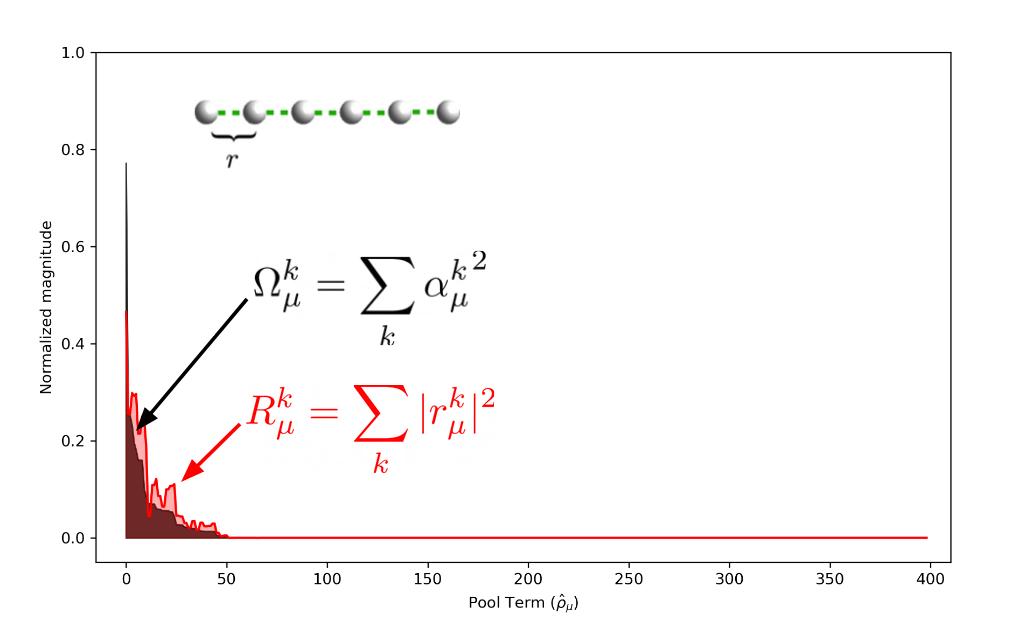
\includegraphics[width=0.45\textwidth]{sqite_paper/full_pool_plot.png}
\caption{Comparison of the accumulated residual magnitudes $R_\mu$ versus the accumulated QITE parameter magnitudes $A_\mu$ for all second-quantized operators in $\mathcal{P}_{\rm{sq}}^{\rm{all}}$ for the H6 chain system. The strong correlation between these two distributions indicates that residual-based selection effectively identifies the same dominant operators as those that ultimately acquire large QITE amplitudes.}
\label{fig:residual_param_comparison}
\end{figure}

% Because we are also interested in low-lying excited states, we partition the overall transformation into two parts, 
% \[
% \hat{U}_n = \hat{U}_n^{\mathrm{QITE}} \, \hat{U}_n^{\mathrm{CIS}},
% \]
% where the first circuit $\hat{U}_n^{\mathrm{CIS}}$ transforms $\ket{\Phi_0}$ into the $n$th configuration-interaction singles (CIS) state \cite{}, providing a reasonable zeroth-order approximation to $\ket{\Psi_n}$. The second part, $\hat{U}_n^{\mathrm{QITE}}$, is then adaptively constructed via the QITE procedure described in Section~\ref{sec:aqite_alg_overview}, using the residual-based selection criterion to systematically introduce the most relevant higher-order excitations and de-excitations.


\subsection{Computational resource requirements in QITE}
\label{sec:computational_req}

As emphasized above, QITE is an iterative procedure whereby each iteration $k$ (with $k=1,2,\dots,K$) solves the linear system 
\begin{equation}
\label{eq:lin_sys_rep}
\mathbf{S}^{(k)} \boldsymbol{\alpha}^{(k)} + \mathbf{b}^{(k)} = \mathbf{0}
\end{equation}
to obtain the expansion coefficients $\alpha_\mu^{(k)}$ for the operators $\{\hat{\rho}_\mu^{(k)}\}$ in the pool $\mathcal{P}^{(k)}$. These coefficients then define a short-time unitary
\begin{equation}
\hat{U}(\Delta \beta)^{(k)} 
\;=\;
\prod_{\mu=1}^{M^{(k)}}
e^{-\,i \,\Delta \beta\,\alpha_\mu^{(k)} \,\hat{\rho}_\mu^{(k)}},
\end{equation}
such that the total QITE wave function (starting from a reference state $\ket{\Phi_0}$) is
\begin{equation}
\ket{\Psi_{\rm{QITE}}} 
\;=\;
\prod_{k=1}^{K}
\hat{U}(\Delta \beta)^{(k)} 
\ket{\Phi_0}
\;=\;
\prod_{k=1}^K
\prod_{\mu=1}^{M^{(k)}}
e^{-\,i\,\Delta \beta\,\alpha_\mu^{(k)} \,\hat{\rho}_\mu^{(k)}}
\ket{\Phi_0}.
\end{equation}
Here, $K = \beta/\Delta \beta$ is the total number of imaginary time steps, and each pool $\mathcal{P}^{(k)}$ has size $M^{(k)}$. The cost of performing QITE may be characterized along several axes:

\paragraph{Classical Parameters.}
A central figure of merit is the total number of parameters $\{\alpha_\mu^{(k)}\}$ used in the QITE unitaries across all iterations. Since each QITE step may introduce a new set of $M^{(k)}$ operators, the \textit{total} number of classical parameters is
\begin{equation}
N_{\rm{QITE}} 
\;=\;
\sum_{k=1}^{K} 
M^{(k)}.
\end{equation}
Larger pools (and hence larger $M^{(k)}$) can improve the flexibility of the QITE ansatz but incur heavier computational and measurement burdens. Designing efficient, possibly adaptive, strategies to select $\mathcal{P}^{(k)}$ is therefore crucial to maintaining tractable classical costs.

\paragraph{Measurements of Observables.}
Each QITE iteration requires measuring matrix elements to construct the linear system in Eq.~\eqref{eq:lin_sys_rep}. Concretely, one needs
\begin{equation}
S_{\mu \nu}^{(k)} 
\;=\; 
2 \,\Re \Bigl[ 
\bra{\Phi^{(k)}} 
\,\hat{\rho}_\mu^{(k)} \,\hat{\rho}_\nu^{(k)}
\ket{\Phi^{(k)}}
\Bigr],
\end{equation}
and,
\begin{equation}
b_{\mu}^{(k)}
\;=\;
\Im \Bigl[
\bra{\Phi^{(k)}}\,
\bigl[\hat{H},\,\hat{\rho}_\mu^{(k)}\bigr]
\ket{\Phi^{(k)}}
\Bigr],
\end{equation}
where $\ket{\Phi^{(k)}} \equiv \hat{U}(\Delta \beta)^{(k-1)} \cdots \hat{U}(\Delta \beta)^{(1)} \ket{\Phi_0}$ denotes the current wave function (i.e., the state at the start of the $k$th iteration). The total number of unique \textit{pairwise} products $\hat{\rho}_\mu^{(k)}\hat{\rho}_\nu^{(k)}$ may be on the order of $(M^{(k)})^2$ per iteration, and one must also measure various commutators $\bigl[\hat{H},\hat{\rho}_\mu^{(k)}\bigr]$. Hence, summing over all $k$, the number of distinct observables can become quite large for big pools. 

While straightforward measurement protocols (e.g., measuring each observable individually) could be prohibitively expensive, more advanced methods such as \textit{classical shadows}\cite{huang2020predicting} can compress the measurement overhead. In essence, classical shadows allow one to efficiently estimate many Pauli expectation values simultaneously using randomized measurements and classical post-processing, reducing the exponential blowup in the number of measurement settings.
\note{red}{should the following be moved to section d (motivation to reduce costs)}
Regardless, one wants to minimize the total number of Pauli operators that need to be measured, especially when treating strongly correlated systems on current hardware. This can be accomplished by choosing operator pools and ansatz structures that lead to fewer measurable terms. Our residual-based selection procedure outlined in Section~\ref{sec:selected_qite} builds a dynamic set of optimal excitation/de-excitation operators through evaluation of residual conditions on the quantum register. This greatly reduces the raw number of terms needing measurement (when compared to static pool types), and removes the need for randomized measurements and classical post-processing. 

\note{blue}{Emphasize that reguardless, one wants to minimize the total number of Pauli operators that need to be measured}


\paragraph{Circuit Depth and Gate Counts.}
From a quantum-circuit perspective, each exponential $e^{-\,i\,\Delta \beta\,\alpha_\mu^{(k)} \,\hat{\rho}_\mu^{(k)}}$ is typically decomposed into a small network of multi-qubit gates (e.g., CNOTs) and parameterized single-qubit rotations. If $\hat{\rho}_\mu^{(k)}$ preserves fundamental symmetries (particle number, spin projection, etc.) and is built from low-rank fermionic excitations (e.g., up to doubles), the Trotter block for $e^{-\,i\,\Delta \beta\,\alpha_\mu^{(k)} \,\hat{\rho}_\mu^{(k)}}$ can often be implemented with a bounded number of CNOTs that scales polynomially in the system size. However, this bounded scaling generally breaks down when higher-order excitations (e.g., triples or beyond) are included, as the corresponding operators typically require deeper circuits with a number of CNOTs that grows rapidly with system size.
\note{blue}{Careful, not true if higher order excitations are included}
In the \textit{deepest} QITE circuit (where the largest operator pool is applied), we may have 
\[
\text{(\# CNOTs)} \;\propto\; \sum_{\mu=1}^{M^{(k_\star)}} \!\!\text{cost}(\hat{\rho}_\mu^{(k_\star)}),
\]
where $k_\star$ is the iteration featuring the largest pool. This cost may be further reduced if adjacent exponentials can be merged or commuted.\cite{mcardle2020quantum} Additionally, each operator \(e^{-\,i\,\Delta \beta\,\alpha_\mu^{(k)} \,\hat{\rho}_\mu^{(k)}}\) introduces at least one parameterized rotation gate, and in practice, multiple rotations may be needed to handle real and imaginary parts or to map the fermionic operator into an appropriate qubit representation. Hence, the total number of \textit{parameterized} gates across all steps is also $\mathcal{O}(N_{\rm{QITE}})$, which serves as a proxy for the T-gate cost in a fault-tolerant setting. 

\paragraph{Motivation to Reduce Costs.}
In summary, the resource requirements of QITE scale with (i) the total number of classical parameters $N_{\rm{QITE}}$, (ii) the number of unique observables measured, and (iii) the circuit depth (especially in terms of CNOTs and parameterized rotations). As larger systems with stronger correlations are considered, these costs can quickly become prohibitive. Consequently, much of this work is devoted to devising efficient strategies for \textit{selecting} and \textit{updating} the pool of operators $\{\hat{\rho}_\mu^{(k)}\}$, thereby minimizing $N_{\rm{QITE}}$ while maintaining sufficient accuracy to capture the essential physics. In parallel, improved measurement protocols (e.g., classical shadows) can mitigate overheads from the exponentially growing number of observables. By combining careful operator selection with more efficient measurement and circuit compilation, one aims to push QITE toward practical regimes even for challenging, strongly correlated electronic structure problems.




%\subsection{Sparsity and Compact Operator Pools}
%There is a great deal of flexibility in how one chooses the Pauli product operators that make up the set $\mathcal{P}$. 
%This choice is also important because if greatly impacts the quantum (and classical) resources required for QITE and ultimately determines its usefulness as a hybrid quantum-classical algorithm. 
%For example, setting $\mathcal{P} = \mathcal{Q}$ would result in the need to repeatedly solve linear systems of dimension $4^{N_{\rm{qb}}}$, which scales even more poorly that the dimension of the entire Fock space.
%In previous work there are two distinct ways to dramatically reduce the dimension of $\mathcal{P}$ without significant loss of accuracy.
%%There are (in our opinion) at least two reasonable ways to dramatically reduce the dimension of $\mathcal{P}$ without significant loss of accuracy.
%
%The first strategy, which is described in detail in the original QITE article [Ref.~\citenum{motta2019determining}] is to consider a set of operators $\mathcal{P}_\ell$ specific to each of the $N_\ell$ terms of the Hamiltonian ($\hat{H}_\ell$), rather than a single set for the entire Hamiltonian. They show that this strategy works quite well for geometric $k$--local Hamiltonians for which each term $\hat{H}_\ell$ acts only on the nearest $k$ (or fewer) qubits.      
%Specifically, they choose some domain $D>k$ qubits such that each $\mathcal{P}_\ell$ contains $4^{D}$ operators such that the total number of QITE parameters is approximated by $n N_\ell 4^D$.
%
%The second strategy, which we also employ in this study (as discussed above), is to limit the operators $ \hat{\rho}_\mu$ to only those that preserve particle-number and spin symmetry. 
%Prior work \cite{} has then considered fixed sets $\mathcal{P}_{\rm{sq}}$ of second quantized excitation and de-excitation operators.
%Specific examples include the set of generalized singles and doubles excitation/de-excitation pairs $\mathcal{P}_{\rm{sq}}^{\rm{GSD}}$ (as similar operators comprise the hamiltonian), and only particle-hole single and double excitation/de-excitation pairs $\mathcal{P}_{\rm{sq}}^{\rm{SD}}$ for a given Hartree-Fock reference determinant.
%
%A key feature of this work is to introduce a selection strategy for constructing an \textit{optimal} set, $\widetilde{\mathcal{P}}_{\rm sq}$, of excitation/de-excitation operator pairs based on the residuals of the projected Schr\"odinger equation. Although there are several sensible selection criteria (e.g., $|b_\mu|$ or perturbative energy estimates similar to those used in selected configuration interaction\cite{selectedCI}), here we employ a protocol closely following the work of Stair \textit{et al.}, which is particularly economical in terms of measurement cost. The rationale is grounded in the so-called \textit{residual condition}: for any unitary $\hat{U}_n$ that transforms a single-determinant reference $\ket{\Phi_0}$ (e.g., Hartree--Fock) into the exact eigenstate $\ket{\Psi_n}$, the residuals
%\begin{equation}
%r_\mu = \bra{\Phi_\mu} \hat{U}_n^\dagger f(\hat{H}) \hat{U}_n \ket{\Phi_0}
%\end{equation}
%must vanish for all determinants $\ket{\Phi_\mu}$ once $\ket{\Psi_n}$ is reached. Here $f(\hat{H})$ is any function of the Hamiltonian sharing the same eigenvectors, and $\ket{\Phi_\mu}$ is the determinant obtained by applying the second-quantized operator $\hat{\rho}_\mu$ to $\ket{\Phi_0}$. 
%\textcolor{red}{Careful with $k_\mu$ vs $\rho_\mu$ here}
%In magnitude, $|r_\mu|$ indicates how much the determinant $\ket{\Phi_\mu}$ is under- or overrepresented in the current approximation to $\ket{\Psi_n}$. Thus, including $\hat{\rho}_\mu$ in the QITE unitary is sensible because it directly addresses the residual mismatch, enabling a more accurate approach to the target eigenstate.
%
%In practice, our numerical evidence suggests that summing the magnitudes of these residuals over all QITE iterations, 
%$R_\mu = \sum_{k} \bigl|r_\mu^{(k)}\bigr|$,
%provides a distribution that closely mirrors the accumulated magnitudes of the solution-vector elements,
%$A_\mu = \sum_{k} \bigl| \alpha_\mu^{(k)}\bigr|$,
%for the same set of candidate operators $\mathcal{P}_{\rm{sq}}$. In other words, operators that consistently exhibit large residuals also acquire large QITE parameters across the imaginary time evolution. Theoretically, this similarity can be rationalized by noting that both $r_\mu$ and $x_\mu$ measure departures of the evolving wave function from the exact target state---the former in terms of incomplete representation in the determinant $\ket{\Phi_\mu}$, and the latter in terms of how strongly $\hat{\rho}_\mu$ must act to correct that imbalance.
%
%\begin{figure}[h!]
%\centering
%\includegraphics[width=0.45\textwidth]{residual_vs_parameter_distribution.pdf}
%\caption{Comparison of the accumulated residual magnitudes $R_\mu$ versus the accumulated QITE parameter magnitudes $X_\mu$ for all second-quantized operators in $\mathcal{P}_{\rm{sq}}^{\rm{all}}$. The strong correlation between these two distributions indicates that residual-based selection effectively identifies the same dominant operators as those that ultimately acquire large QITE amplitudes.}
%\label{fig:residual_param_comparison}
%\end{figure}
%
%Because we are also interested in higher-lying states, we partition the overall transformation into two parts, 
%\[
%\hat{U}_n = \hat{U}_n^{\mathrm{QITE}} \, \hat{U}_n^{\mathrm{CIS}},
%\]
%where the first circuit $\hat{U}_n^{\mathrm{CIS}}$ transforms $\ket{\Phi_0}$ into the $n$th configuration-interaction singles (CIS) state \cite{}, providing a reasonable zeroth-order approximation to $\ket{\Psi_n}$. The second part, $\hat{U}_n^{\mathrm{QITE}}$, is then adaptively constructed via the QITE procedure described in Section~\ref{sec:aqite_alg_overview}, using the residual-based selection criterion to systematically introduce the most relevant higher-order excitations and de-excitations.



%In our approach, we first consider some set ($\mathcal{P}_{\rm{sq}}$) of second quantized excitation and de-excitation operators, a reasonable choice is the set of generalized singles and doubles excitation/de-excitation pairs (as these operators comprise the hamiltonian).
%\textcolor{red}{use equation here and below}
%Another is to consider only particle-hole single and double excitation/de-excitation pairs for a given hartree-fock reference. 
%\textcolor{red}{We note that both of these approaches have been considered in prior work CITE.}
%For each individual second quantized operator in ($\mathcal{P}_{\rm{sq}}$) we consider the group of Pauli operators obtained via the Jordan-Wigner transformation.
%We then add all unique Pauli operators ($\hat{\rho}_\mu$) found in this way to the set $\mathcal{P}$.
%$\mathcal{P}$ is then farther truncated to include only Pauli operators that contain an odd number of $\hat{\sigma}_Y$'s because (for real wave functions) Eq.~\eqref{eq:qite2} can only be satisfied when $\Im \big( \bra{\Phi} \hat{\rho}_\mu^\dagger \hat{H} \ket{\Phi} \big)$ and $\Re \big( \bra{\Phi} \hat{\rho}_\mu^\dagger  \hat{\rho}_\nu \ket{\Phi} \big)$ are non-zero.

\note{red}{NOTE: Think about selection for excited states as well.}

%\subsection{QITE with Low Rank Hamiltonians}
%Another way to exploit sparsity in the evolution is by considering low rank factorization of...

\section{Computational Details}
The ground-state singlet energies and molecular integrals of the H10 model systems were calculated using FCI with self consistent field (SCF) orbitals obtained with the open-source quantum chemistry package Psi4 \cite{Parrish2017Psi4, smith2020psi4} in a STO-6G basis set. For the two ene systems (8-ene, 12-ene), The ground-state singlet energies and molecular integrals were calculated using FCI within an active space among the Carbon atom 2pz orbitals automatically selected through AVAS~\cite{sayfutyarova2017automated} using the open-source quantum chemistry package PySCF \cite{sun2018pyscf}. All ground state computations were performed in C1 symmetry. \note{red}{To respond to this point: "It says we used C1 symmetry for everything, but you may have used d2h symmetry on some of the hydrogen systems?" I am actually not sure since I didnt specify symmetry when running the psi4 calculations} The ranges of threshold parameters used for sQITE are given in the Supplementary Material. Tsuchimochi et al previously reported that a second-order derivation of the QITE equations avoids first-order dependence on time step, $\Delta\beta$, even at large time step of $\Delta\beta$ = 0.1 \cite{Tsuchimochi2023Improved}. Currently, we have found that convergence can be reached at time steps as large as $\Delta\beta$ = 0.5, allowing for a significant reduction in resource usage for a second order derivation of QITE. 

\begin{figure}[h!]
\centering
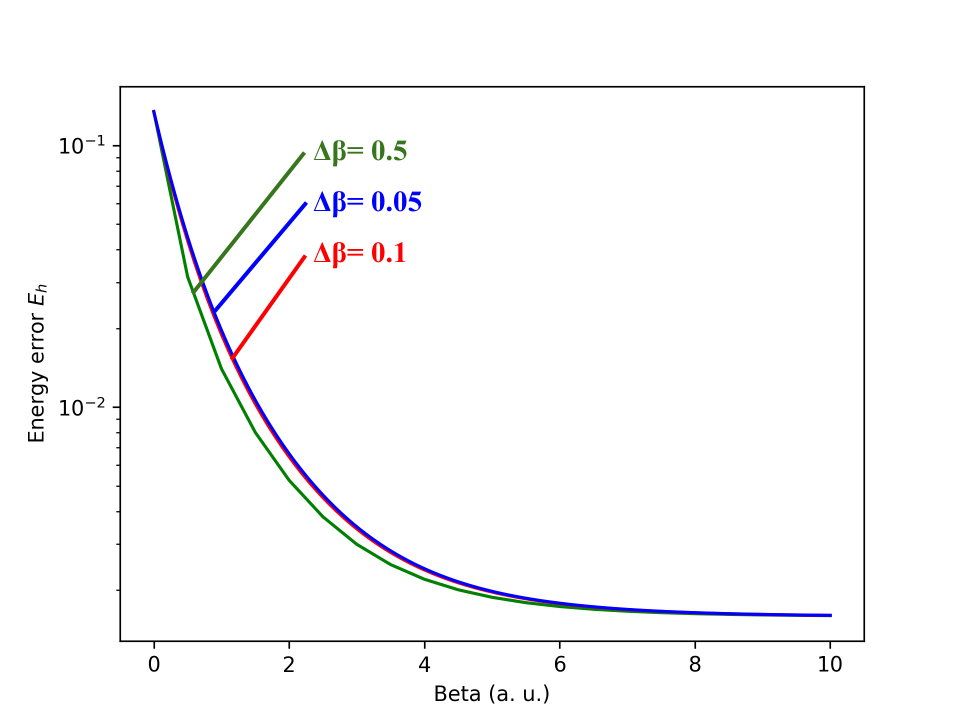
\includegraphics[width=0.45\textwidth]{sqite_paper/paper_db_plot.png}
\caption{dUCCSD energy convergence for the H8 chain system at 1.0 Å bond distance at different time steps $\Delta\beta$ = 0.5, 0.1, 0.05. We find no discernable difference between the final energy error of QITE runs with different timesteps in a singles and doubles UCCSD Ansatz propagated from the same Hartree-Fock initial state.}
\label{fig:db_plot_1.0A}
\end{figure}

Further resource reduction can be accomplished through our double-factorization scheme, and through usage of a range of truncation thresholds, we found up to an order of magnitude reduction in cumulative cnot gate depths. All ene systems were run with the same double-factorized threshold.

In this study, we utilized double-factorized Hamiltonians to reduce circuit depths associated with residual overhead from the selection procedure. To generate these Hamiltonians for time evolution, we employed helper functions from the OpenFermion\cite{mcclean2020openfermion} library as well as the fermionic-quantum-emulator.\cite{rubin2021fermionic} Although the implementation resides within the QForte framework, the underlying code for double factorization and related transformations was directly adapted from these two libraries. Computations were performed in a development version of the open-source quantum simulation and chemistry library QForte \cite{stair2021qforte}. 


\note{blue}{write about how double factorization employs d2H symmetry here}


% Canonical (delocalized) orbitals were computed usingrestricted Hartree–Fock (RHF). Localized orbitals were obtained by first performing a restricted open-shell Hartree-Fock (ROHF) computation using maximum multiplicity (e.g., S = 5for H10) and then localizing the orbitals with the Pipek–Mezey(PM)133 procedure (allowing rotations among all orbitals).

% Computations based on canonical RHF orbitals were run in D2h symmetry for the H10 chain, ring, and sheet and in C2v symmetry for the H10 pyramid. The H12, H14, and H16 analogs of the four systems were run with the same symmetry as their H10 counterparts with the exception of the H14 pyramid, which used D2h symmetry. All computations using localized orbitals were performed in C1 symmetry. The ranges of threshold parameters used for each method are given in the Supplementary Material.

% All ACI computations included additional determinants to ensure spin completeness of the P and Q spaces. The rank-reduction procedure used for SVD-FCI and the a posteriori determinant screening procedure for ap-sCI were implemented in a development version of Forte. 

% Density matrix renormalization group calculations were performed with CheMPS2.145 DMRG calculations associated with a particular final value of M were preceded by three preliminary computations with smaller bond dimension and added noise. This procedure has been shown to make the overall DMRG calculation converge more rapidly and produce more accurate results.78,146 In the first two preliminary computations M is set to 150, 500, 500, and 500 (for H10, H12,H14, and H16 respectively) to build an initialization for the last two instructions with a larger value of M. In cases where the final value of M is less than the values specified above, the same value of M is used for the three preliminary calculations and for the final calculation. As mentioned already, due to the block structure of the DMRG tensors induced by symmetries, the final MPS in general does not correspond to a set of dense matrices of dimension M2. For DMRG calculations using a localized basis, orbitals for the 1D chain and ring were ordered to be spatially consecutive. Localized orbitals for the 2D sheet and 3D pyramid systems used a Fiedler vector ordering derived from the two electron integrals to account fo physical proximity and orbital overlap.82 Plots of the localized orbitals and the site orderings are reported in the Supplementary Material. For canonical MOs, orbitals were grouped into blocks by irreducible representation and (within each irreducible representation) ordered energetically. For calculations using D2h symmetry, the irreducible representation blocks were ordered as Ag, B1u, B3u, B2g, B2u, B3g, B1g, Au such that blocks corresponding to bonding and anti-bonding orbitals were adjacent on the DMRG lattice. This strategy has been shown to be successful for several DMRG studies81,147–149 and is rationalized by quantum information principles.119 For calculations using symmetries other than D2h, the ordering of the irreducible representations followed Cotton’s ordering.

\section{Results}
To evaluate the efficiency of the selected Quantum Imaginary Time Evolution (sQITE) approach relative to standard quantum algorithms, we performed numerical simulations on several molecular systems of increasing complexity, specifically three hydrogen systems (H$_{10}$ chain, ring, and sheet geometries) at bond lengths of 1.0 Å and 1.5 Å, as well as larger conjugated organic systems, 8-ene and 12-ene.

% \begin{figure}[h!]
% \centering
% 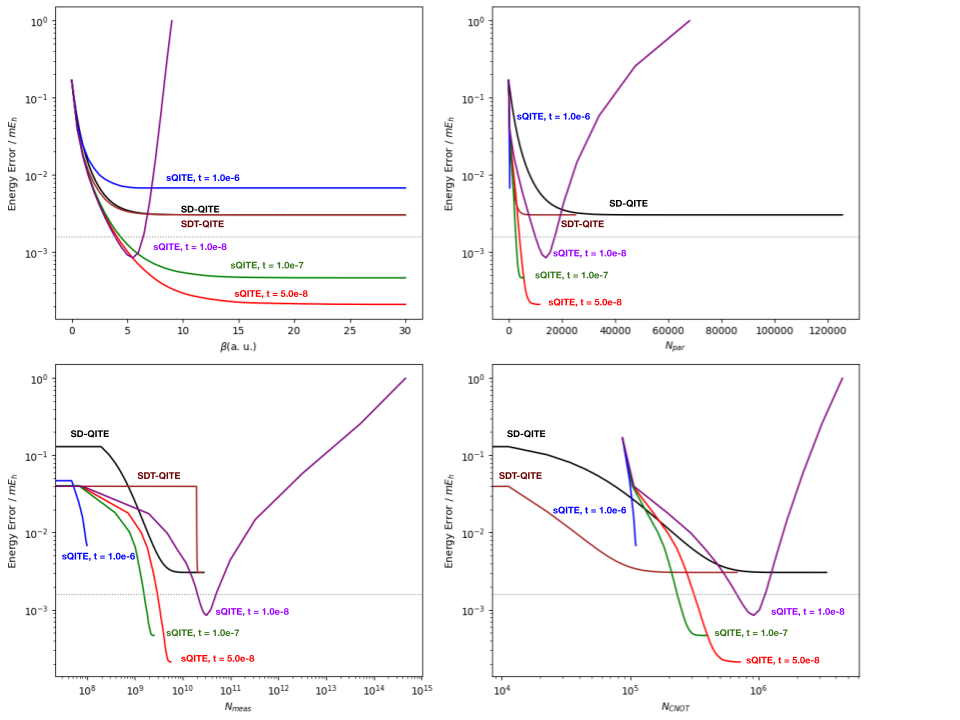
\includegraphics[width=0.45\textwidth]{sqite_paper/Chain 1.0 A.png}
% % 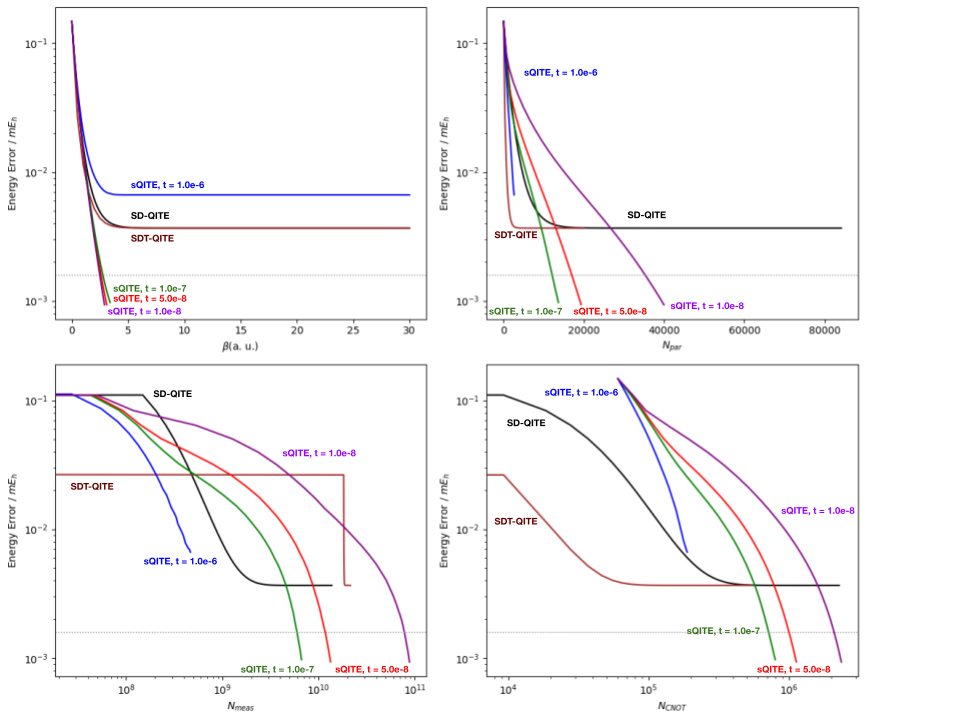
\includegraphics[width=0.45\textwidth]{sqite_paper/Ring 1.0 A.png}
% 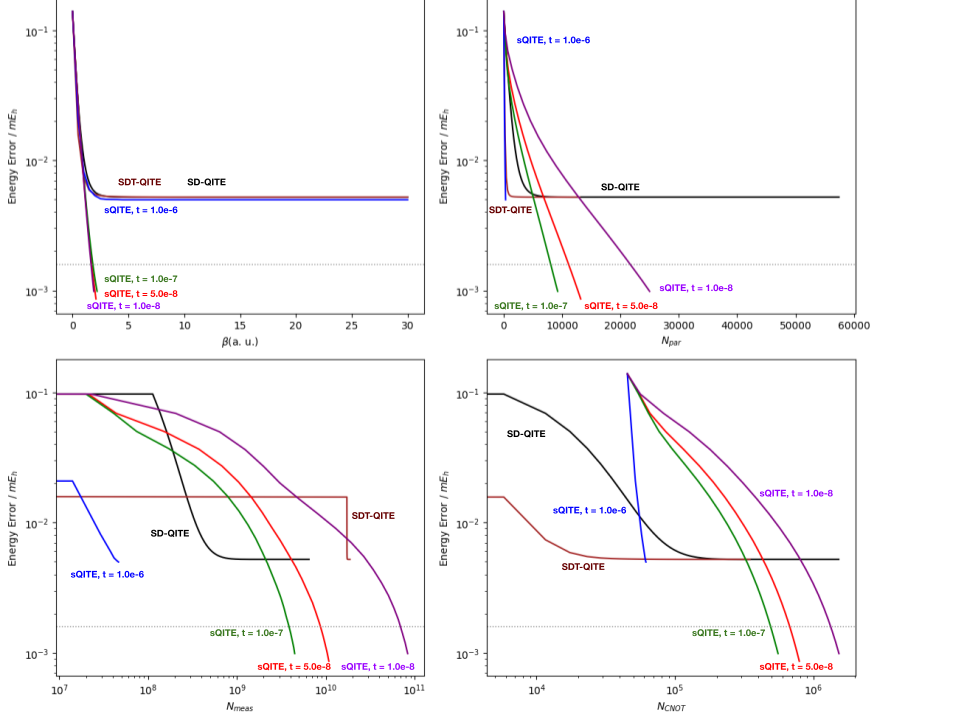
\includegraphics[width=0.45\textwidth]{sqite_paper/Sheet 1.0 A.png}
% \caption{dUCCSD energy convergence for H10 systems (chain, sheet) at 1.0 Å bond distance. We show the absolute value of the energy change between subsequent iterations for QITE in a singles and doubles UCC Ansatz, a singles doubles ad triples UCC Ansatz, and selected QITE with 4 different cumulative thresholds ($1.0 \times 10^{-6}$, $1.0 \times 10^{-7}$, $5.0 \times 10^{-8}$, $1.0 \times 10^{-8}$ $E_h$) for relative operator magnitudes. All plots compare convergence with respect to the number of Pauli measurements ($N_\mathrm{meas}$), number of CNOT gates ($N_\mathrm{CNOT}$), number of classical parameter ($N_\mathrm{par}$), and evolution amount ($\beta (a. u.)$).}
% \label{fig:ene_plot_1.0A}
% \end{figure}

\begin{figure*}[htbp]
\centering
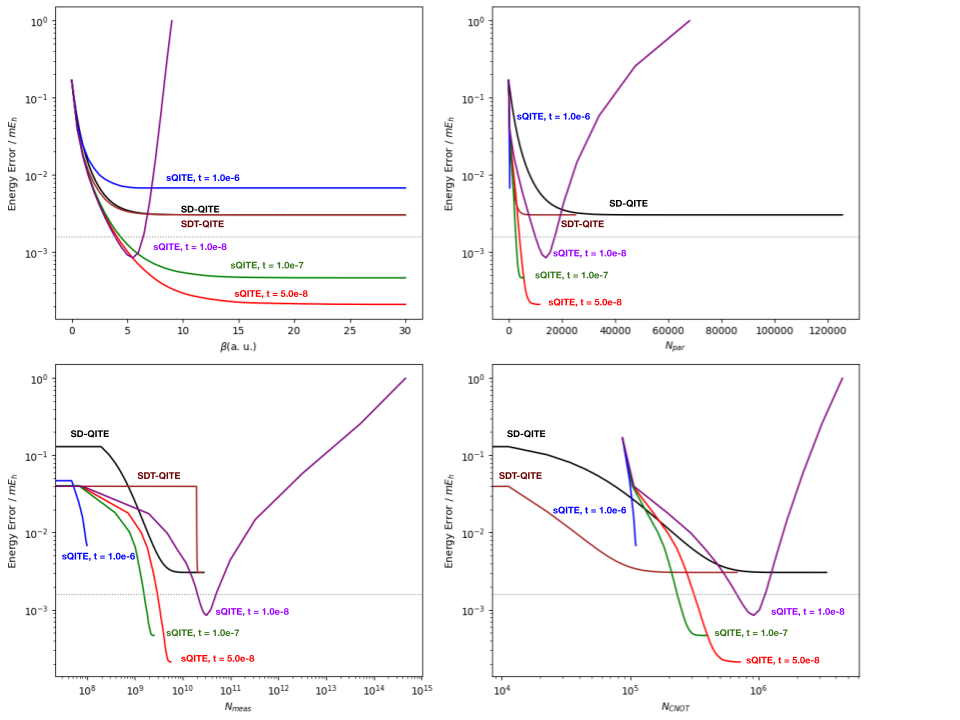
\includegraphics[width=0.48\textwidth]{sqite_paper/Chain 1.0 A.png}
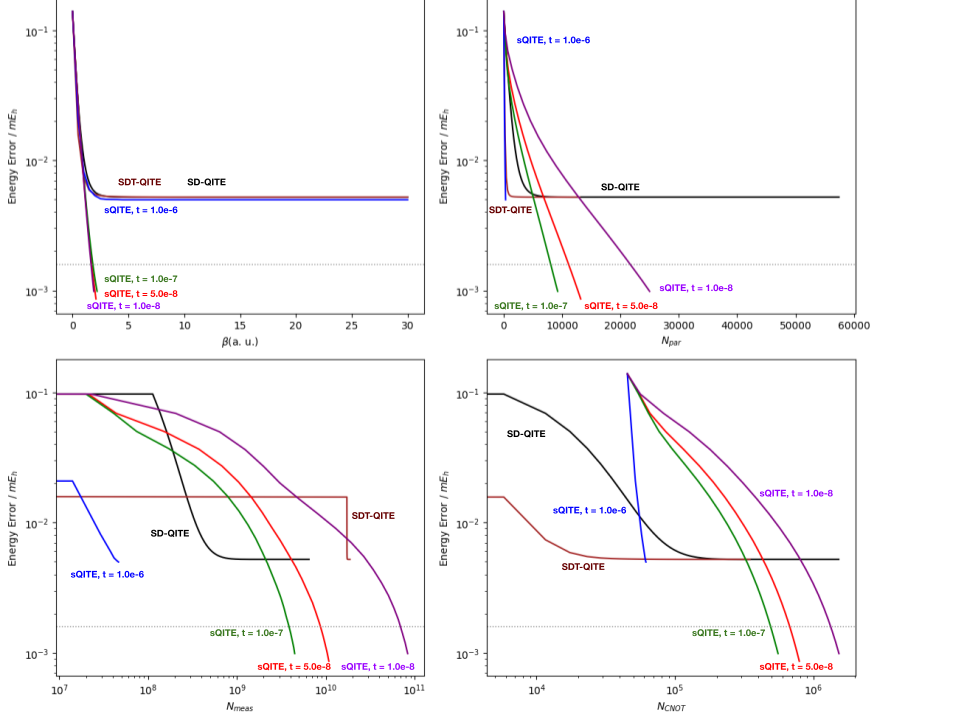
\includegraphics[width=0.48\textwidth]{sqite_paper/Sheet 1.0 A.png}
\vspace{1em} % Optional vertical space between rows
% Uncomment the next lines if you have additional plots
% 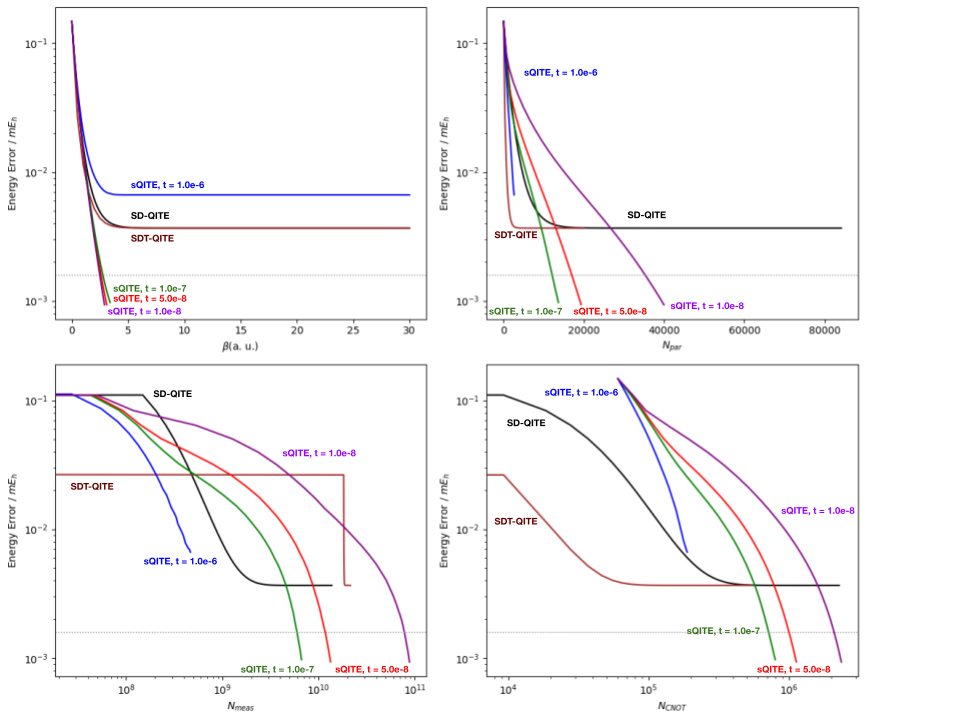
\includegraphics[width=0.48\textwidth]{sqite_paper/Ring 1.0 A.png}
% \includegraphics[width=0.48\textwidth]{sqite_paper/AnotherPlot.png}
\caption{dUCCSD energy convergence for H10 systems (chain, sheet) at 1.0 Å bond distance. We show the absolute value of the energy change between subsequent iterations for QITE in a singles and doubles UCC Ansatz, a singles doubles ad triples UCC Ansatz, and selected QITE with 4 different cumulative thresholds ($1.0 \times 10^{-6}$, $1.0 \times 10^{-7}$, $5.0 \times 10^{-8}$, $1.0 \times 10^{-8}$ $E_h$) for relative operator magnitudes. All plots compare convergence with respect to the number of Pauli measurements ($N_\mathrm{meas}$), number of CNOT gates ($N_\mathrm{CNOT}$), number of classical parameter ($N_\mathrm{par}$), and evolution amount ($\beta (a. u.)$).}
\label{fig:ene_plot_1.0A}
\end{figure*}

% \begin{figure}[h!]
% \centering
% 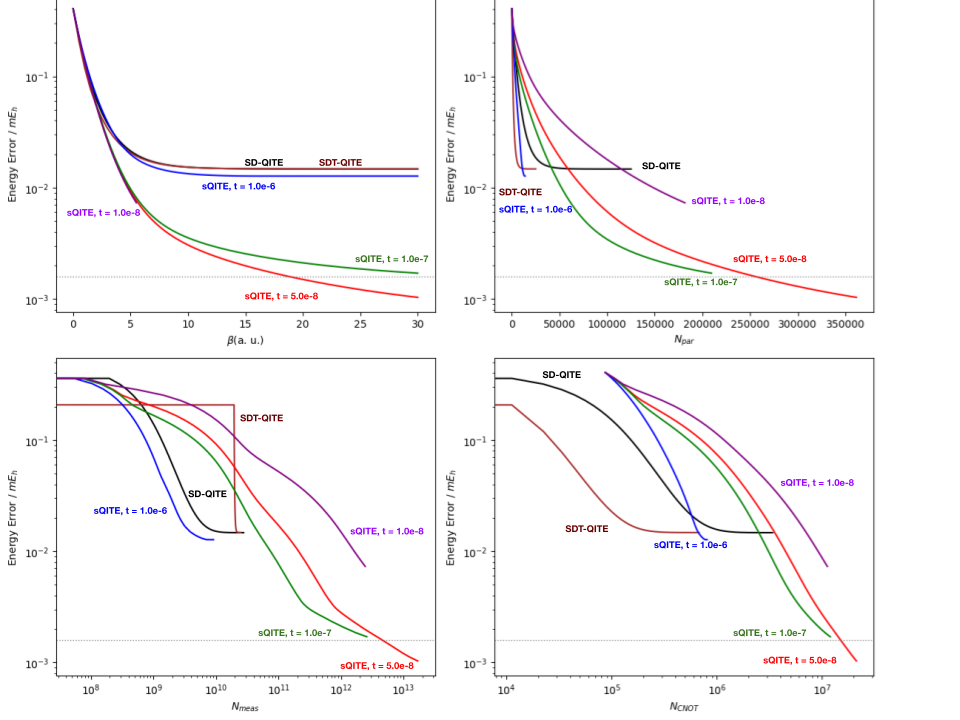
\includegraphics[width=0.45\textwidth]{sqite_paper/Chain 1.5 A.png}
% 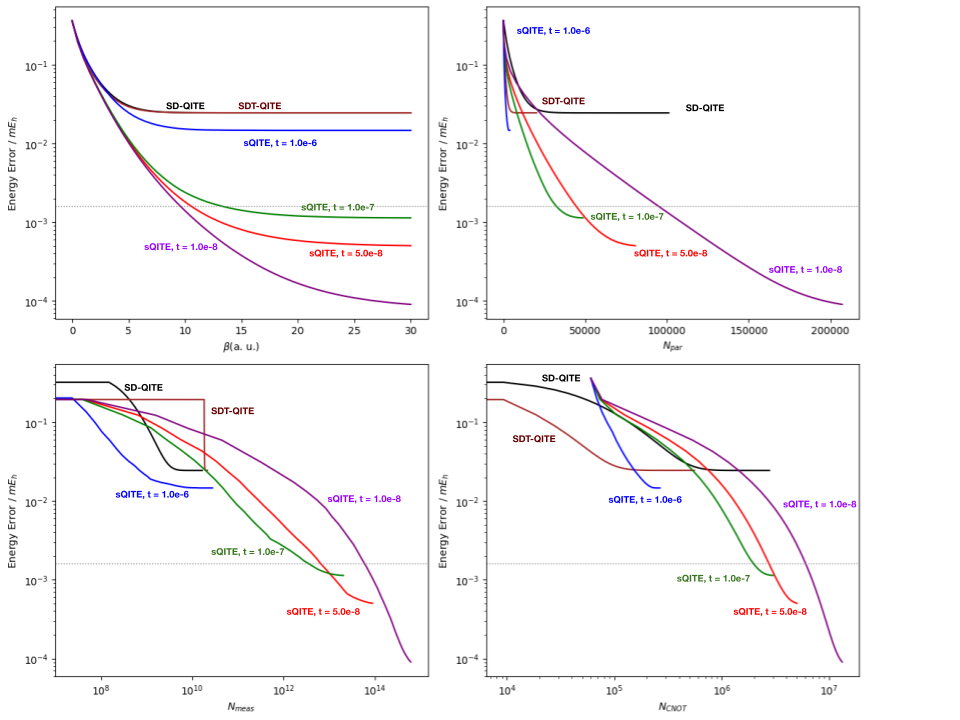
\includegraphics[width=0.45\textwidth]{sqite_paper/Ring 1.5 A.png}
% 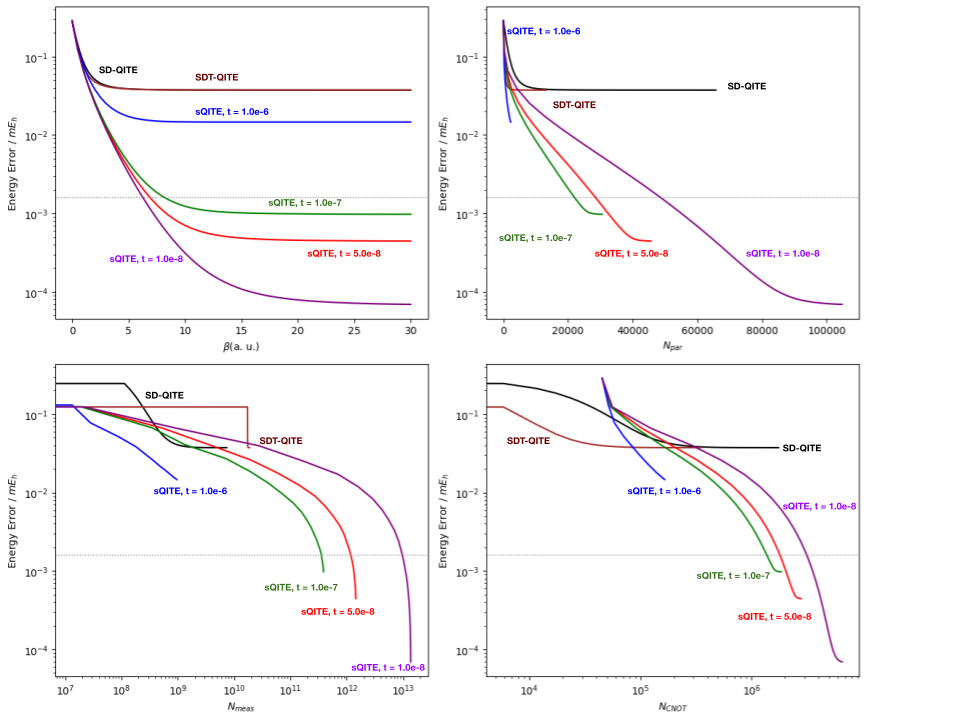
\includegraphics[width=0.45\textwidth]{sqite_paper/Sheet 1.5 A.png}
% \caption{dUCCSD energy convergence for H10 systems (chain, ring, sheet) at 1.5 Å bond distance. We show the absolute value of the energy change between subsequent iterations for QITE in a singles and doubles UCC Ansatz, a singles doubles ad triples UCC Ansatz, and selected QITE with 4 different cumulative thresholds ($1.0 \times 10^{-6}$, $1.0 \times 10^{-7}$, $5.0 \times 10^{-8}$, $1.0 \times 10^{-8}$ $E_h$) for relative operator magnitudes. All plots compare convergence with respect to the number of Pauli measurements ($N_\mathrm{meas}$), number of CNOT gates ($N_\mathrm{CNOT}$), number of classical parameter ($N_\mathrm{par}$), and evolution amount ($\beta (a. u.)$).}
% \label{fig:ene_plot_1.5A}
% \end{figure}

% \begin{figure}[h!]
% \centering
% 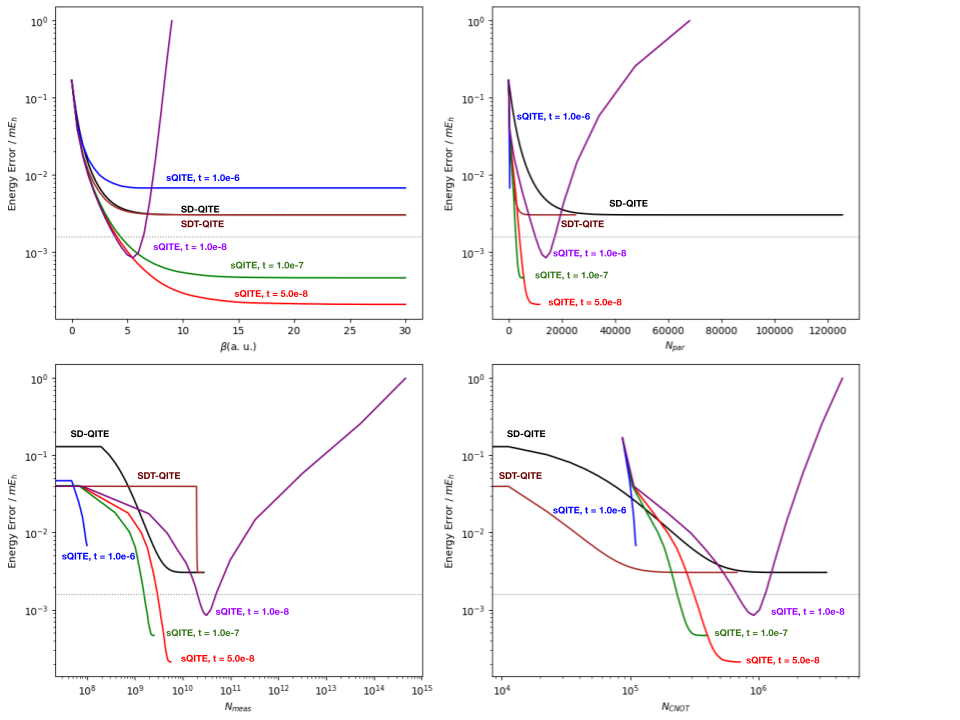
\includegraphics[width=0.45\textwidth]{sqite_paper/Chain 1.0 A.png}
% \\
% 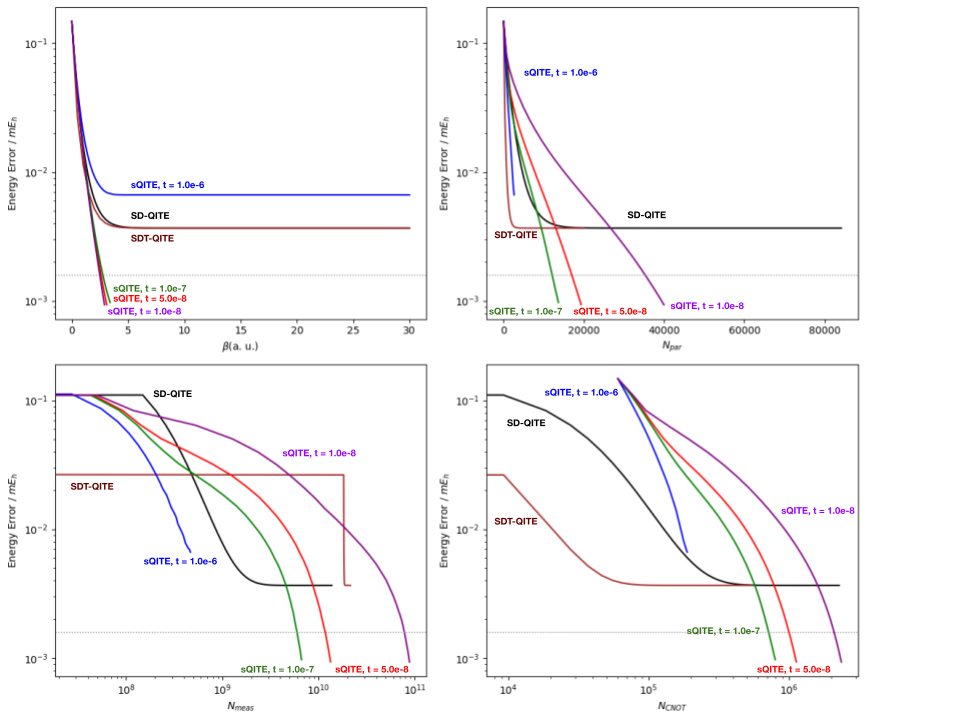
\includegraphics[width=0.45\textwidth]{sqite_paper/Ring 1.0 A.png}
% \\
% 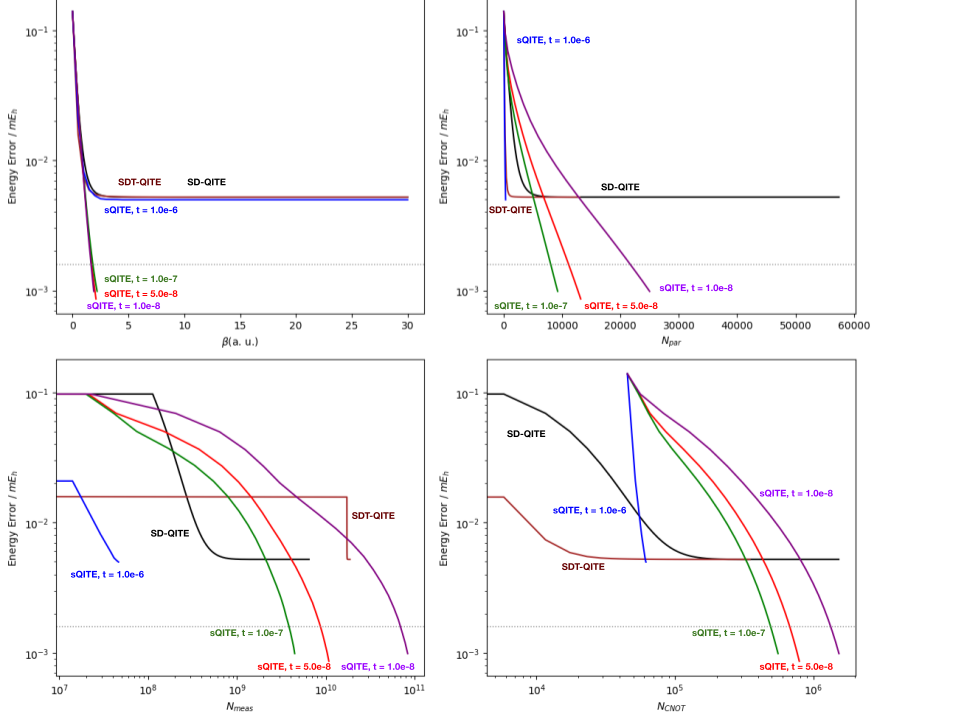
\includegraphics[width=0.45\textwidth]{sqite_paper/Sheet 1.0 A.png}
% \\
% 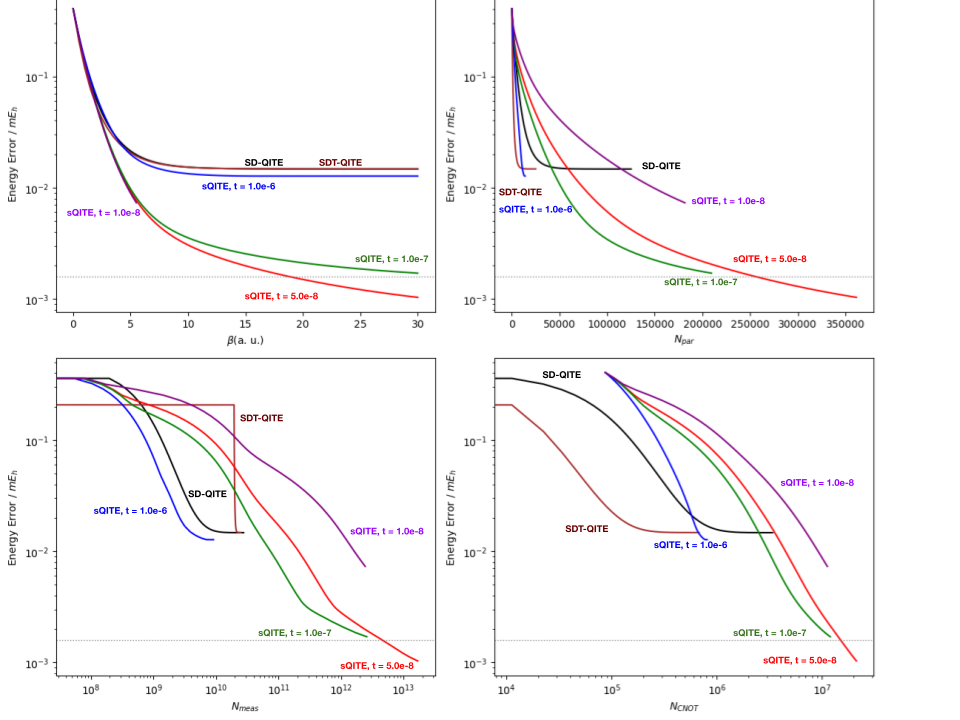
\includegraphics[width=0.45\textwidth]{sqite_paper/Chain 1.5 A.png}
% \\
% 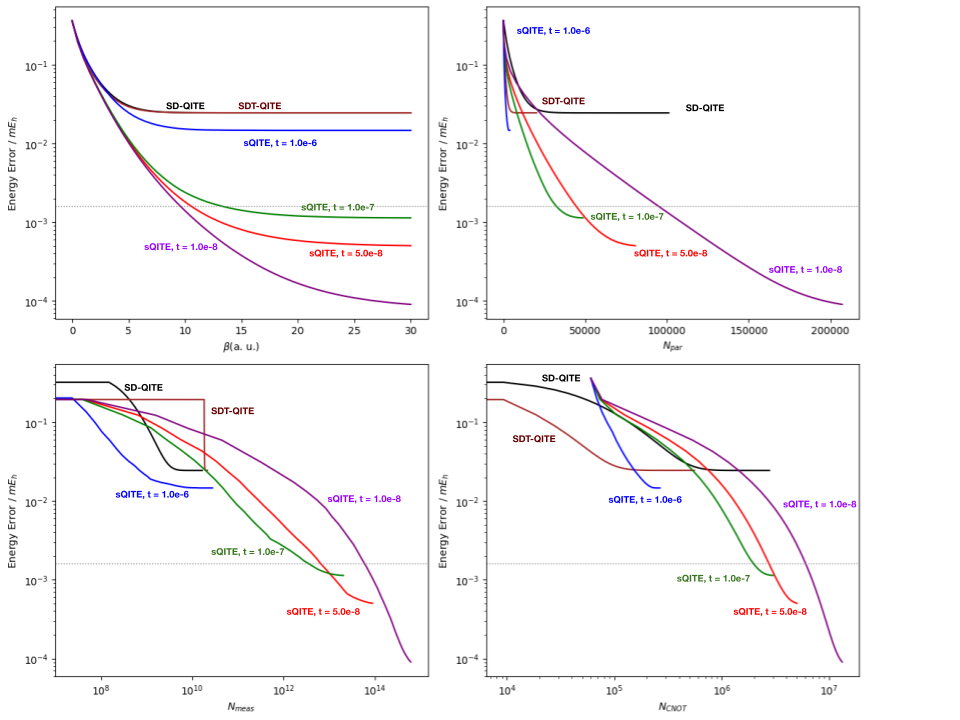
\includegraphics[width=0.45\textwidth]{sqite_paper/Ring 1.5 A.png}
% \\
% 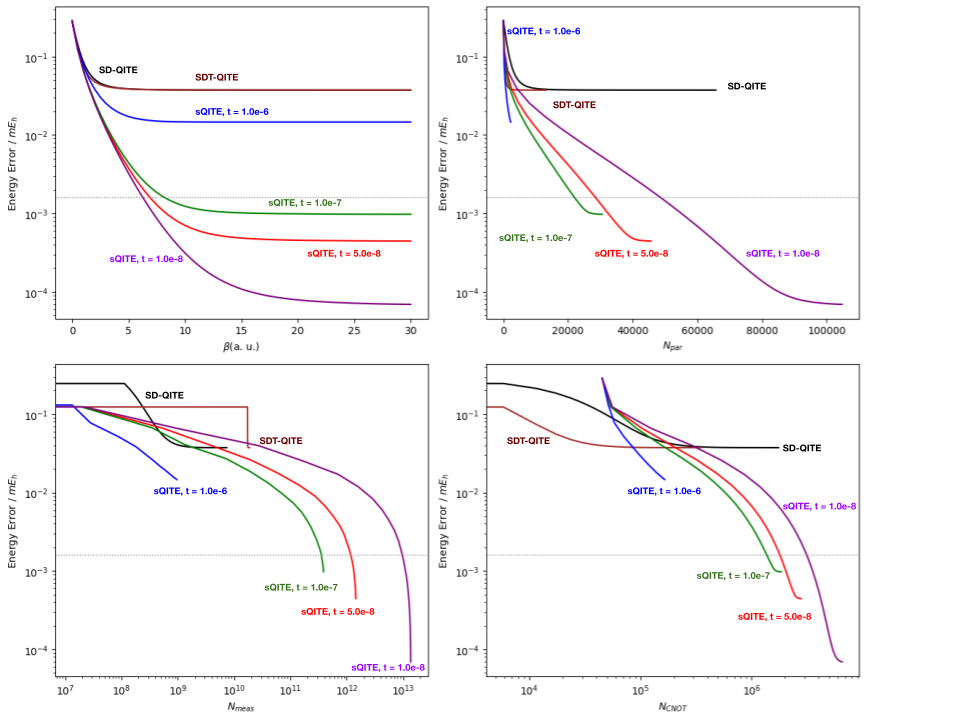
\includegraphics[width=0.45\textwidth]{sqite_paper/Sheet 1.5 A.png}
% \caption{dUCCSD energy convergence for H10 model hydrogen systems (chain, ring, sheet) at 1.0 and 1.5 angstrom bond distances. We show the absolute value of the energy change between subsequent iterations for QITE in a singles and doubles UCC Ansatz, a singles doubles ad triples UCC Ansatz, and selected QITE with 4 different cumulative thresholds ($1.0 \times 10^{-6}$, $1.0 \times 10^{-7}$, $5.0 \times 10^{-8}$, $1.0 \times 10^{-8}$ $E_h$) for relative operator magnitudes. All plots compare convergence with respect to the number of Pauli measurements ($N_\mathrm{meas}$), number of CNOT gates ($N_\mathrm{CNOT}$), number of classical parameter ($N_\mathrm{par}$), and evolution amount ($\beta (a. u.)$).}
% \label{fig:ene_plot}
% \end{figure}

We first analyzed the number of Pauli measurements required to achieve chemical accuracy, defined as an energy error of less than 1.6 mHartree, for different operator inclusion thresholds. Boths plots below display the results for the chain and sheet hydrogen systems at the 1.0 Å bond length, clearly indicating that certain operator thresholds allow sQITE to achieve chemical accuracy with significantly fewer Pauli measurements compared to the fixed singles and doubles pool approach. This result highlights the advantages of a dynamically selected operator pool.

In addition, we assessed the complexity of quantum circuits by counting CNOT gates required for chemical accuracy, also presented below. Consistent with our findings for Pauli measurements, the sQITE algorithm outperforms the fixed singles and doubles pool in terms of gate complexity at certain thresholds, demonstrating the method's capability to reduce quantum resource requirements substantially.

For example, in the H\textsubscript{10} chain at 1.0 \AA{}, sQITE achieved convergence within one order of magnitude to chemical accuracy using up to 100× fewer Pauli measurements and 2× fewer CNOT gates compared to fixed-ansatz QITE, while also requiring fewer classical parameters. Moreover, while fixed-ansatz QITE consistently failed to reach chemical accuracy in strongly correlated regimes (e.g., stretched geometries at 1.5 angstrom), sQITE was able to do so reliably by selectively adapting the operator pool based on a carefully chosen threshold value. This demonstrates both resource efficiency and accuracy improvements enabled by the selection procedure.

% Finally, we estimated classical resource overhead by tracking the cumulative dimension of the linear system solved each time step by the QITE algorithm. Consistent with our findings for quantum resource costs, the sQITE algorithm outperforms fixed pools and other hybrid quantum/classical algorithms such as SPQE and ADAPT-VQE, due to a combination of reduced scaling in the dynamic pool and the simplicity of the linear system.

Furthermore, a direct comparison between regular sQITE, and double-factorized sQITE was conducted on the 8-ene system. Double factorized sQITE consistently provided reduced circuit depths among a range of thresholds, achieving chemical accuracy with fewer quantum resources. The comprehensive analysis is summarized in Figure~\ref{fig:df_plot_ene}. This plot clearly indicates that double factorization significantly reduces resource requirements, achieving cost efficiency with only negligible accuracy losses compared to regular sQITE. This enhancement underscores the utility of double factorization for larger and strongly correlated molecular systems.
\begin{figure}[h!]
\centering
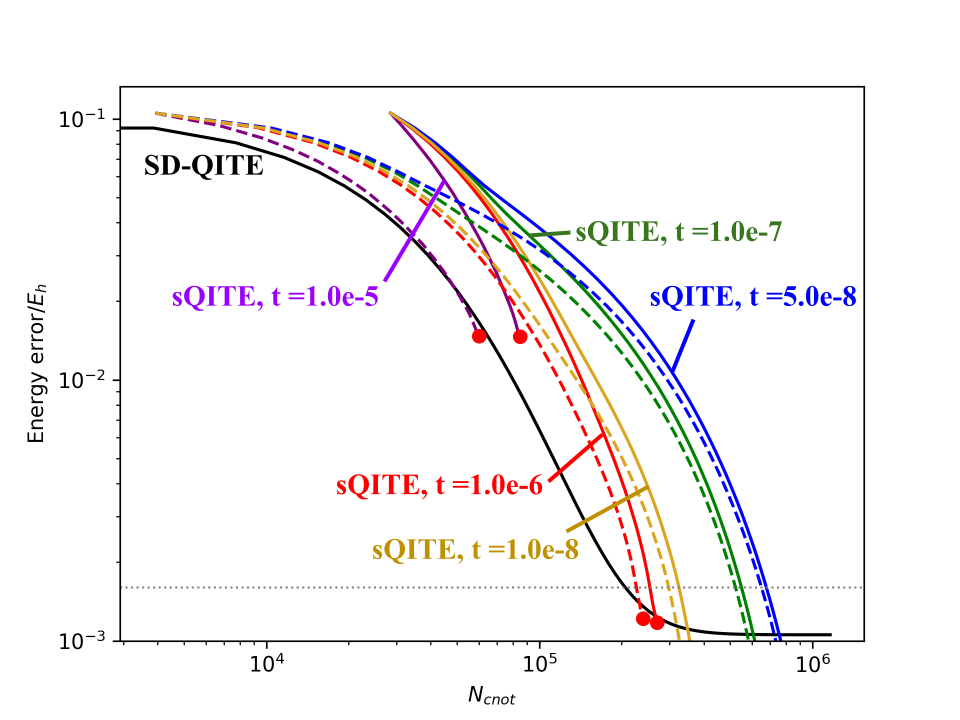
\includegraphics[width=0.45\textwidth]{sqite_paper/paper_df_ham_plot.png}
\caption{dUCCSD energy convergence for 8-ene chains in a cc-pVDZ basis using AVAS among 2pz orbitals of carbon. We demonstrate that a reduction in quantum circuit depths through double-factorization of the residual state does not result in loss of accuracy for the final QITE energy. runs of dfQITE (dotted lines) are plotted against QITE in a singles and doubles UCC Ansatz, and sQITE with 5 different cumulative thresholds ($1.0 \times 10^{-5}$, $1.0 \times 10^{-6}$, $1.0 \times 10^{-7}$, $5.0 \times 10^{-8}$, $1.0 \times 10^{-8}\ E_h$) for relative operator magnitudes. Plot compares convergence with respect to the number of CNOT gates ($N_\mathrm{CNOT}$). \textcolor{blue}{change CNOT resource estimation to count cnot full before regenerating data}}
\label{fig:df_plot_ene}
\end{figure}

For the same hydrogen systems at an extended bond length of 1.5 Å, we demonstrate a similar trend in the efficiency of the sQITE algorithm. Both the Pauli measurements and CNOT gates required to reach chemical accuracy were significantly lower for selected operator pools compared to fixed operator approaches, reflecting sQITE's consistent performance across different molecular geometries and bond distances.

We extended our analysis to larger molecular systems, specifically the conjugated hydrocarbons 8-ene and 12-ene. Figures \ref{fig:ene_plot_1.0A} and \ref{fig:df_plot_ene} demonstrates that sQITE again substantially reduces the number of Pauli measurements, classical parameters, and CNOT gates necessary to reach chemical accuracy compared to fixed pools, confirming its scalability to larger systems.

% \begin{figure}[h!]
% \centering
% 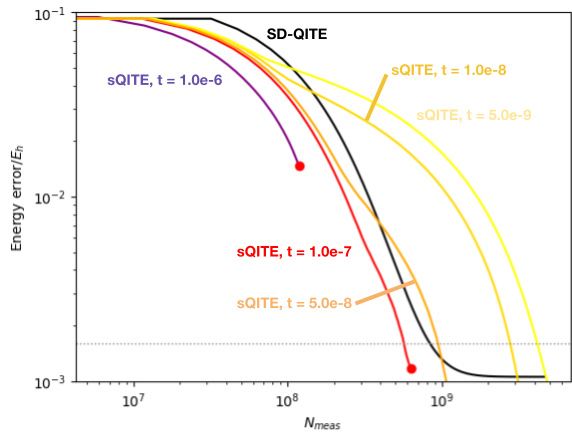
\includegraphics[width=0.45\textwidth]{sqite_paper/ene_plot_SD_v_selected.png}
% \\
% 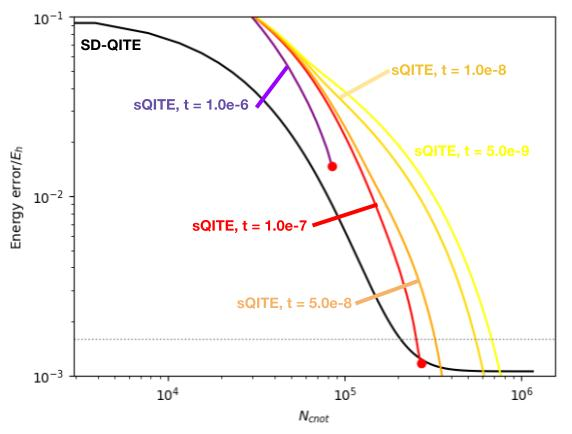
\includegraphics[width=0.45\textwidth]{sqite_paper/ene_plot_cnot.jpg}
% \caption{dUCCSD energy convergence for 8-ene chains in a cc-pVDZ basis using AVAS among 2pz orbitals of carbon. We show the absolute value of the energy change between subsequent iterations for QITE in a singles and doubles UCC Ansatz, and selected QITE with 5 different cumulative thresholds ($1.0 \times 10^{-6}$, $1.0 \times 10^{-7}$, $5.0 \times 10^{-8}$, $1.0 \times 10^{-8}$, $5.0 \times 10^{-9}\ E_h$) for relative operator magnitudes. Both plots compare convergence with respect to the number of Pauli measurements ($N_\mathrm{meas}$) and number of CNOT gates ($N_\mathrm{CNOT}$).}
% \label{fig:ene_plot}
% \end{figure}

In summary, these results demonstrate the robustness, efficiency, and accuracy of the selected QITE approach in conjunction with double-factorized Hamiltonians. The significant reductions in required Pauli measurements and CNOT gates across diverse molecular systems and bond geometries indicate that selected QITE represents a viable and powerful quantum algorithm, potentially outperforming fixed pool methods in resource-limited quantum computing environments.
\section{Conclusions}
In this work, we introduced a dynamically adaptive operator selection strategy for Quantum Imaginary Time Evolution (sQITE), significantly improving the resource efficiency for quantum simulations of electronic structure problems. By leveraging residual-based selection from a comprehensive operator pool, we demonstrated marked reductions in the number of Pauli measurements, classical parameters, and quantum gates—particularly CNOT gates—without compromising chemical accuracy.

Through numerical simulations on hydrogen chains, rings, sheets, and larger conjugated hydrocarbons (8-ene and 12-ene), we showed that sQITE consistently outperformed static operator pool methods and hybrid quantum-classical algorithms, providing robust performance across diverse molecular systems and bond geometries. Additionally, integrating a double-factorization scheme further compressed measurement overhead and circuit complexity, solidifying sQITE as an exceptionally resource-effective method suitable for near-term quantum devices.

Looking forward, our results underscore the potential of adaptive strategies to mitigate computational demands inherent to quantum algorithms for strongly correlated electrons. Future extensions could explore combining sQITE with advanced measurement techniques, error mitigation, and enhanced circuit compilation strategies, potentially expanding its applicability to more complex molecular and materials systems, thereby accelerating progress toward practical quantum chemical simulations.

\bibliography{bibliography,extra}

\end{document}

























